Due to the immense computational requirements of this analysis and that of \parencite{Lee2022MeasurementDetector}, efforts were directed in parallel to investigating enhancing the simulation pipeline with statistical methods. In particular, normalizing flows were examined as a way to reduce computational needs for correction factor determinations, as well as for assisting in solving inverse problems. 

The event generation described earlier in this chapter can be posed as generating a 16xn truth-level dataset, where n is the number of DV$\pi^0$P events produced, with each event containing four 4-vectors to yield 16 elements of information \footnote{The conventions of this work are the first four features (0-3) to represent the electron 4-vector, the next four (4-7) the proton's, and then the two photons, with the higher energy photon ordered first (features 8-11). }. This information must be transformed in a realistic way into the four-momenta typically observed after event reconstruction, data processing, and exclusivity cuts are applied. Traditionally this is achieved through the simulation processing described in previous sections, involving swimming each particle through microphysics simulations and applying reconstruction algorithims to the resulting simulated detector hits. 

Normalizing flows are generative models that are trained to transform distributions that are easy to sample from (like a standard Gaussian) into complex distributions from which sampling is difficult or unknown. Several groups in particle physics are utilizing normalizing flows, for example, training flows to reduce LHC simulation time \parencite{Weisser2021ThePhysics} or work at MIT's IAIFI focused on speeding up aspects of Lattice QCD by a factor of up to 1,000 \parencite{Kanwar2020EquivariantTheory}. The initial motivation for this study was to explore a simliar speedup - sampling from a simple distribution and transforming it into a realistic output event could be significantly faster than than swimming particles through the exact physics fields of the modeled experiment, allowing for a vast amount of computing resources to be saved.  
    
\subsection{Inverse Transforms and Autoregressive Flows}
    
    Normalizing flow are effective models to learn a probability distribution $p(x)$ when a sample data set $X=\{x\}$ following the distribution is given. The basic idea is a series of transformation $g_i$'s, which are referred to as flows, transforms a prior probability $p(z)$ distributions into the target distribution $p(x)$. That is
    \begin{align}
        \mathbf{x} =& g_N \circ g_{N-1}\circ ... \circ g_1 (\mathbf{z}), \\
        \mathbf{z} =& f_1 \circ ... \circ f_{N-1} \circ f_N (\mathbf{x}), \label{eqn:invertible}
    \end{align}
    where $f_{N-i+1}\equiv g_i^{-1}$ following \parencite{Kobyzev2021NormalizingMethods}'s convention. Both $\mathbf{x}$ and $\mathbf{z}$ are vectors of the same dimension $d$. From the eq.~\ref{eqn:invertible}, $g_i$ requires an invertibility condition. An intermediate flow $\mathbf{z_i}$ is defined as follows.
    \begin{align}
    \mathbf{z_i} =&g_i \circ ... \circ g_1(\mathbf{z}), \label{eqn:forward}\\
        =&f_{i+1}\circ ...f_N(\mathbf{x}), \label{eqn:backward}
    \end{align}
    where the flow is expressed in forward direction at eq.~\ref{eqn:forward}, and in backward direction at eq.~\ref{eqn:backward}. Therefore, $\mathbf{z_{i+1}}=g_i (\mathbf{z_i})$ and $\mathbf{z_i} = f_{N-i+1}(\mathbf{z_{i+1}})$ for one flow, or layer. If the $f_i$'s are differentiable, the PDF evolves as follows.
    \begin{align}
     p(\mathbf{z_{i+1}})=& p(\mathbf{z_i})|\frac{\partial f_{N-i+1}}{\partial \mathbf{z_i}}| =p(\mathbf{z_i})|\frac{\partial g_{i}^{-1}}{\partial \mathbf{z_i}}|\\
     \log p(\mathbf{z_{i+1}}) =& \log p(\mathbf{z_i}) + \log|\frac{\partial g_i^{-1}}{\partial \mathbf{z_i}}| \label{eqn:logprob}\\
     \log p(\mathbf{x}) =& \log p(\mathbf{z}) + \sum\limits_{i=1}^N \log|\frac{\partial g_i^{-1}}{\partial \mathbf{z_i}}|.
    \end{align}
    Eq.~\ref{eqn:logprob} is useful to define the forward and the backward propagation of each layer.
    Once the NF model is trained to learn the distribution $g: p(z)\rightarrow p(x)$, it is possible to sample $x$ using sampled $z$. \parencite{Gao2020EventFlows} showed that the Nonlinear Independent Component Estimation (NICE) \parencite{Dinh2014NICE:Estimation} implementation of NF performs well by comparing the technique to existing methods in terms of efficiencies that are defined as average weight during the generation.

\subsection{Exploration of Simulation Speedup with UNMAF}

    Motivated by \parencite{Weisser2021ThePhysics}'s work, Masked Autoregressive Flows were used for this investigation (MAF)  \parencite{Papamakarios2017MaskedEstimation}, which is one of the generalized versions of NICE. The MAF starts from a simple fact that $p(z_{i}) = \prod\limits_{j}p(z_{i,j}|\mathbf{z}_{i,0:j-1})$. The component $z_{i,j}$ is the $j$-th component of $z_i$, and the vector $\mathbf{z}_{i,0:j-1}$ is defined as $\{z_{i, 0}, ..., z_{i, j-1}\}$. The transformation is finally defined as
    \begin{align}
        z_{i+1, j}=& \sigma_{i, j} z_{i, j} + \mu_{i+1, j}.
    \end{align}
    The moments $\mu_{i+1, j}$ and $\sigma_{i, j}$ are the mean and standard deviation of $p(z_{i+1,j}|\mathbf{z}_{i+1,0:j-1})$ ($\equiv p(z_{i+1,0})$ for $j=0$). We train the flows to learn $\mu_{i+1, j}$'s and $\sigma_{i, j}$'s, and sample $p(\mathbf{x})$. 

    More specifically, Unconstrained Monotonic Neural Networks (UMNN-MAF), \parencite{Wehenkel2019UnconstrainedNetworks}  architecture was utilized, as it is able to learn noncontinuous distributions from stacked data files. \parencite{Wehenkel2019UnconstrainedNetworks} demonstrates that the UMNN-MAF successfully learn discontinuous distributions, and that sampling is possible even in the case that the transformation is not analytically invertible.
    
    A training set of 5M data points was generated and processed using the traditional simulation tools discussed earlier in this chapter. This yielded a training input vector $\mathbf{x}$ with dimensions of $5\text{M}\times16$, where each element is just a floating point number.

    \subsubsection*{Architecture and Training}
        Models were trained on the full 16 feature data set as well as on 4 feature subsets (corresponding to single particle mappings). Our architecture consisted of 16 layers of UMNN-MAF with 32 hidden variables per layer in the 16-feature case, and consisted of 6 layers with 80 hidden variables per layer in the 4-feature case. After many trials of different combinations of hyper parameters and flow models, we found that an effective training method to use a maximum of 10K epochs, with each iteration using randomly sampled training data sets of 400$\times$16 dimension from the initial 5M data points generated by physics simulations. In practice, only several hundred epochs were needed for convergence; see \figref{fig:jul8_pion_comparison4}. To evaluate our model, we sampled 100k data points, $\mathbf{x_1}$, from the physics simulation set which were not included in training, and generated 100k data points, $\mathbf{x_2}$, using our trained model.The Earth Mover's Distance (EMD), calculable as the Wasserstein-1 Distance \parencite{Dobrushin1970PrescribingDistributions} was evaluate between $\mathbf{x_1}$ and $\mathbf{x_2}$. 
        
        Training the NF models was relatively fast, for the 16-feature model taking about 1 hour on a GPU (NVIDIA Quadro RTX 5000) or about 10 hours on a CPU (Intel Xeon E-2276M). On the other hand, sampling from the trained model was considerably slower; the 16-feature trained NF model generated datapoints at a rate of about 4 Hz, which is only a factor of 10 times faster than the traditional method of simulating the processes' microphysics. 
        
        \parencite{Wehenkel2019UnconstrainedNetworks} and \parencite{Papamakarios2017MaskedEstimation} explains this behavior as follows. The Masked Autoencoder for Distribution Estimation (MADE, \parencite{Germain2015MADE:Estimation}), which is a building block of MAF allows the training to be done in parallel using GPUs. Sampling data points from the trained MAF takes significant amount of time because the model requires $\mathbf{z}_{i,0:j-1}$ to sample $\mathbf{z}_{i,j}$. There is a computational trade-off in Inverse Autoregressive Flow (IAF, \parencite{Kingma2016ImprovingFlow}, which trains the model slowly but samples fast. 

    
        To improve training, all features were transformed to quantile distributions. Formally, given a random variable $X$ and its cumulative distribution function $F$, the transformed variable $X^*$ is defined as $X^* = F^{-1}(F(X))$, where $F^{-1}$ is the quantile function of the target distribution. \ref{fig:quantile_transforms} displays the effect on sample feature distributions. 

        %I.e. "from sklearn.preprocessing import QuantileTransformer"
        
        \begin{figure}[H]
            \centering
            \begin{minipage}{.3\textwidth}
            
                \centering
               % Electron
                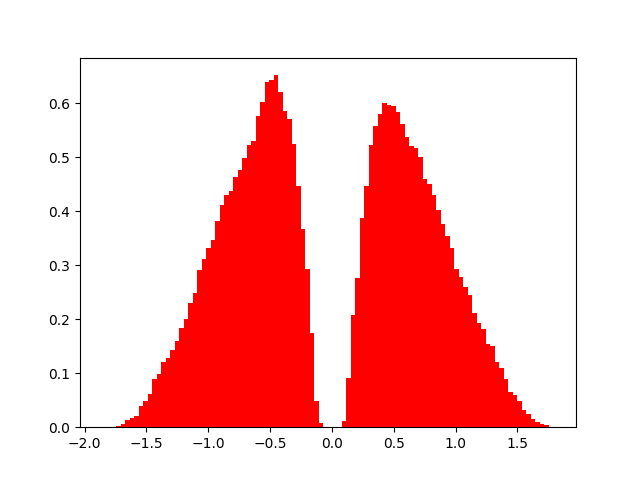
\includegraphics[width=.99\textwidth,trim={3cm 0 0 0},clip]{Chapters/Ch3-Simulations/normalizing_flows/pics/MeetingFigures/Bobby/QT/feature0_noQT.png}
                %\caption[Placeholder Short text]{(a)}
                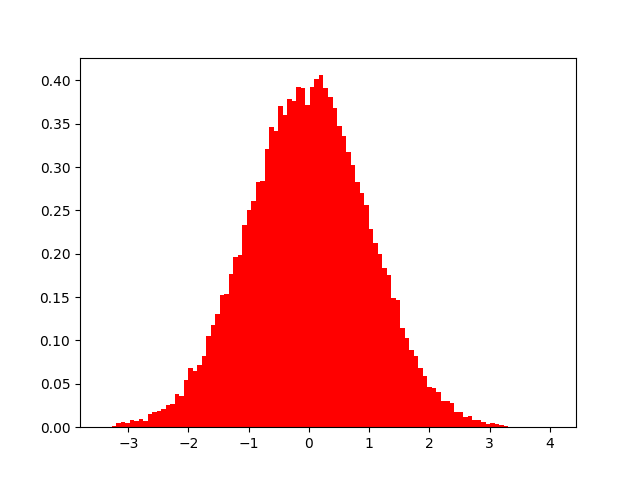
\includegraphics[width=.99\textwidth,trim={3cm 0 0 0},clip]{Chapters/Ch3-Simulations/normalizing_flows/pics/MeetingFigures/Bobby/QT/feature0.png}
        
                %\caption[Placeholder Short text]{(c)}
            \end{minipage}%
            \begin{minipage}{.3\textwidth}
            
                \centering
               % Electron
                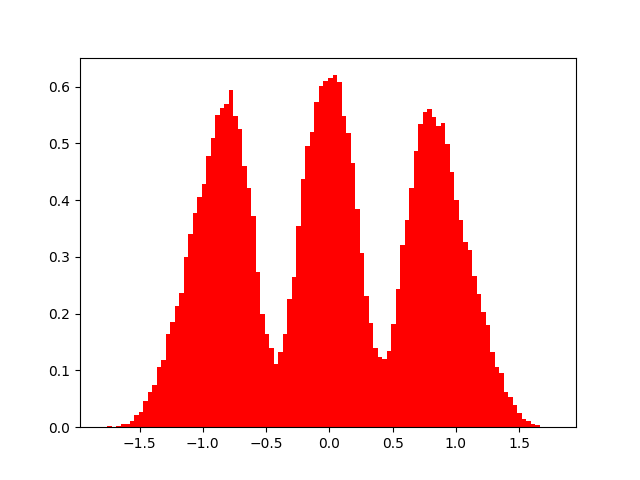
\includegraphics[width=.99\textwidth,trim={3cm 0 0 0},clip]{Chapters/Ch3-Simulations/normalizing_flows/pics/MeetingFigures/Bobby/QT/feature1_noQT.png}
                %\caption[Placeholder Short text]{(a)}
                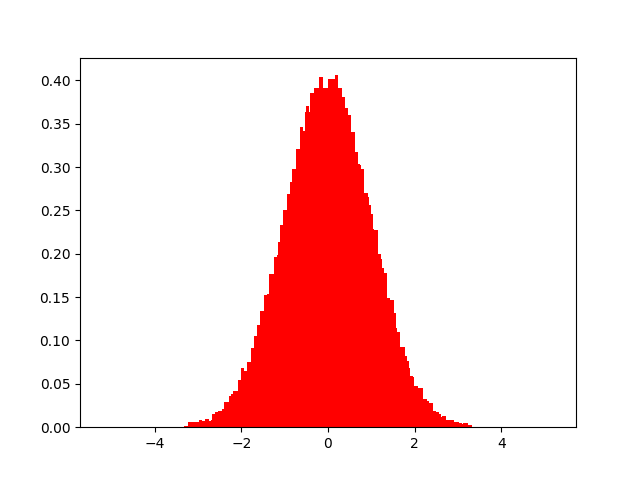
\includegraphics[width=.99\textwidth,trim={3cm 0 0 0},clip]{Chapters/Ch3-Simulations/normalizing_flows/pics/MeetingFigures/Bobby/QT/feature1.png}
        
                %\caption[Placeholder Short text]{(c)}
            \end{minipage}%
            \begin{minipage}{.3\textwidth}
            
                \centering
               % Electron
                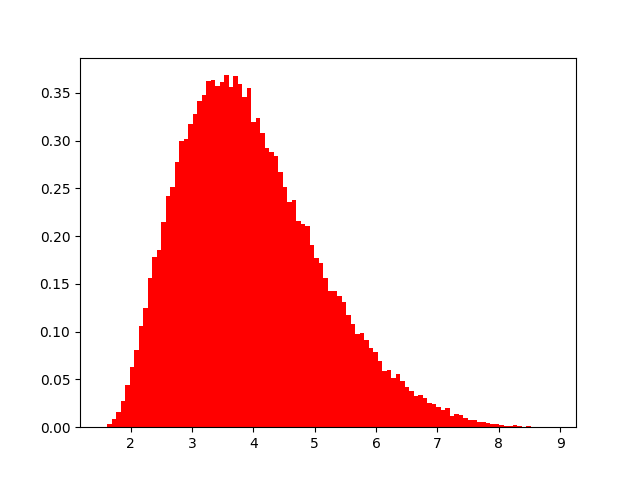
\includegraphics[width=.99\textwidth,trim={3cm 0 0 0},clip]{Chapters/Ch3-Simulations/normalizing_flows/pics/MeetingFigures/Bobby/QT/feature2_noQT.png}
                %\caption[Placeholder Short text]{(a)}
                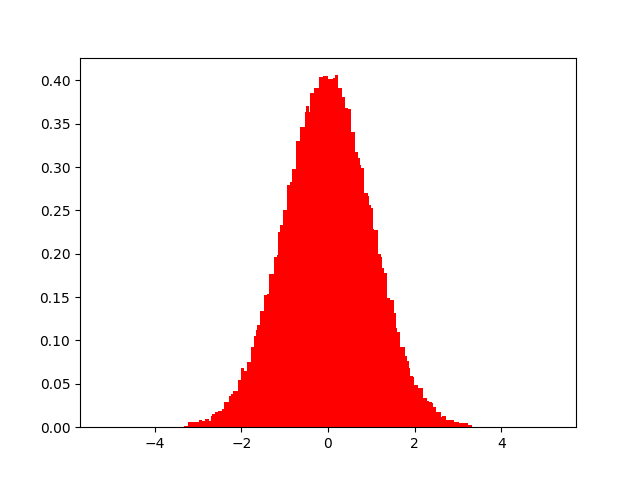
\includegraphics[width=.99\textwidth,trim={3cm 0 0 0},clip]{Chapters/Ch3-Simulations/normalizing_flows/pics/MeetingFigures/Bobby/QT/feature2.png}
        
                %\caption[Placeholder Short text]{(c)}
            \end{minipage}%
            \caption[Data Pre-processing Quantile Transforms]{Sample feature distributions before (top) and after (bottom) quantile transforms}
            \label{fig:quantile_transforms}
        \end{figure}


        \begin{figure}[H]
            \centering
            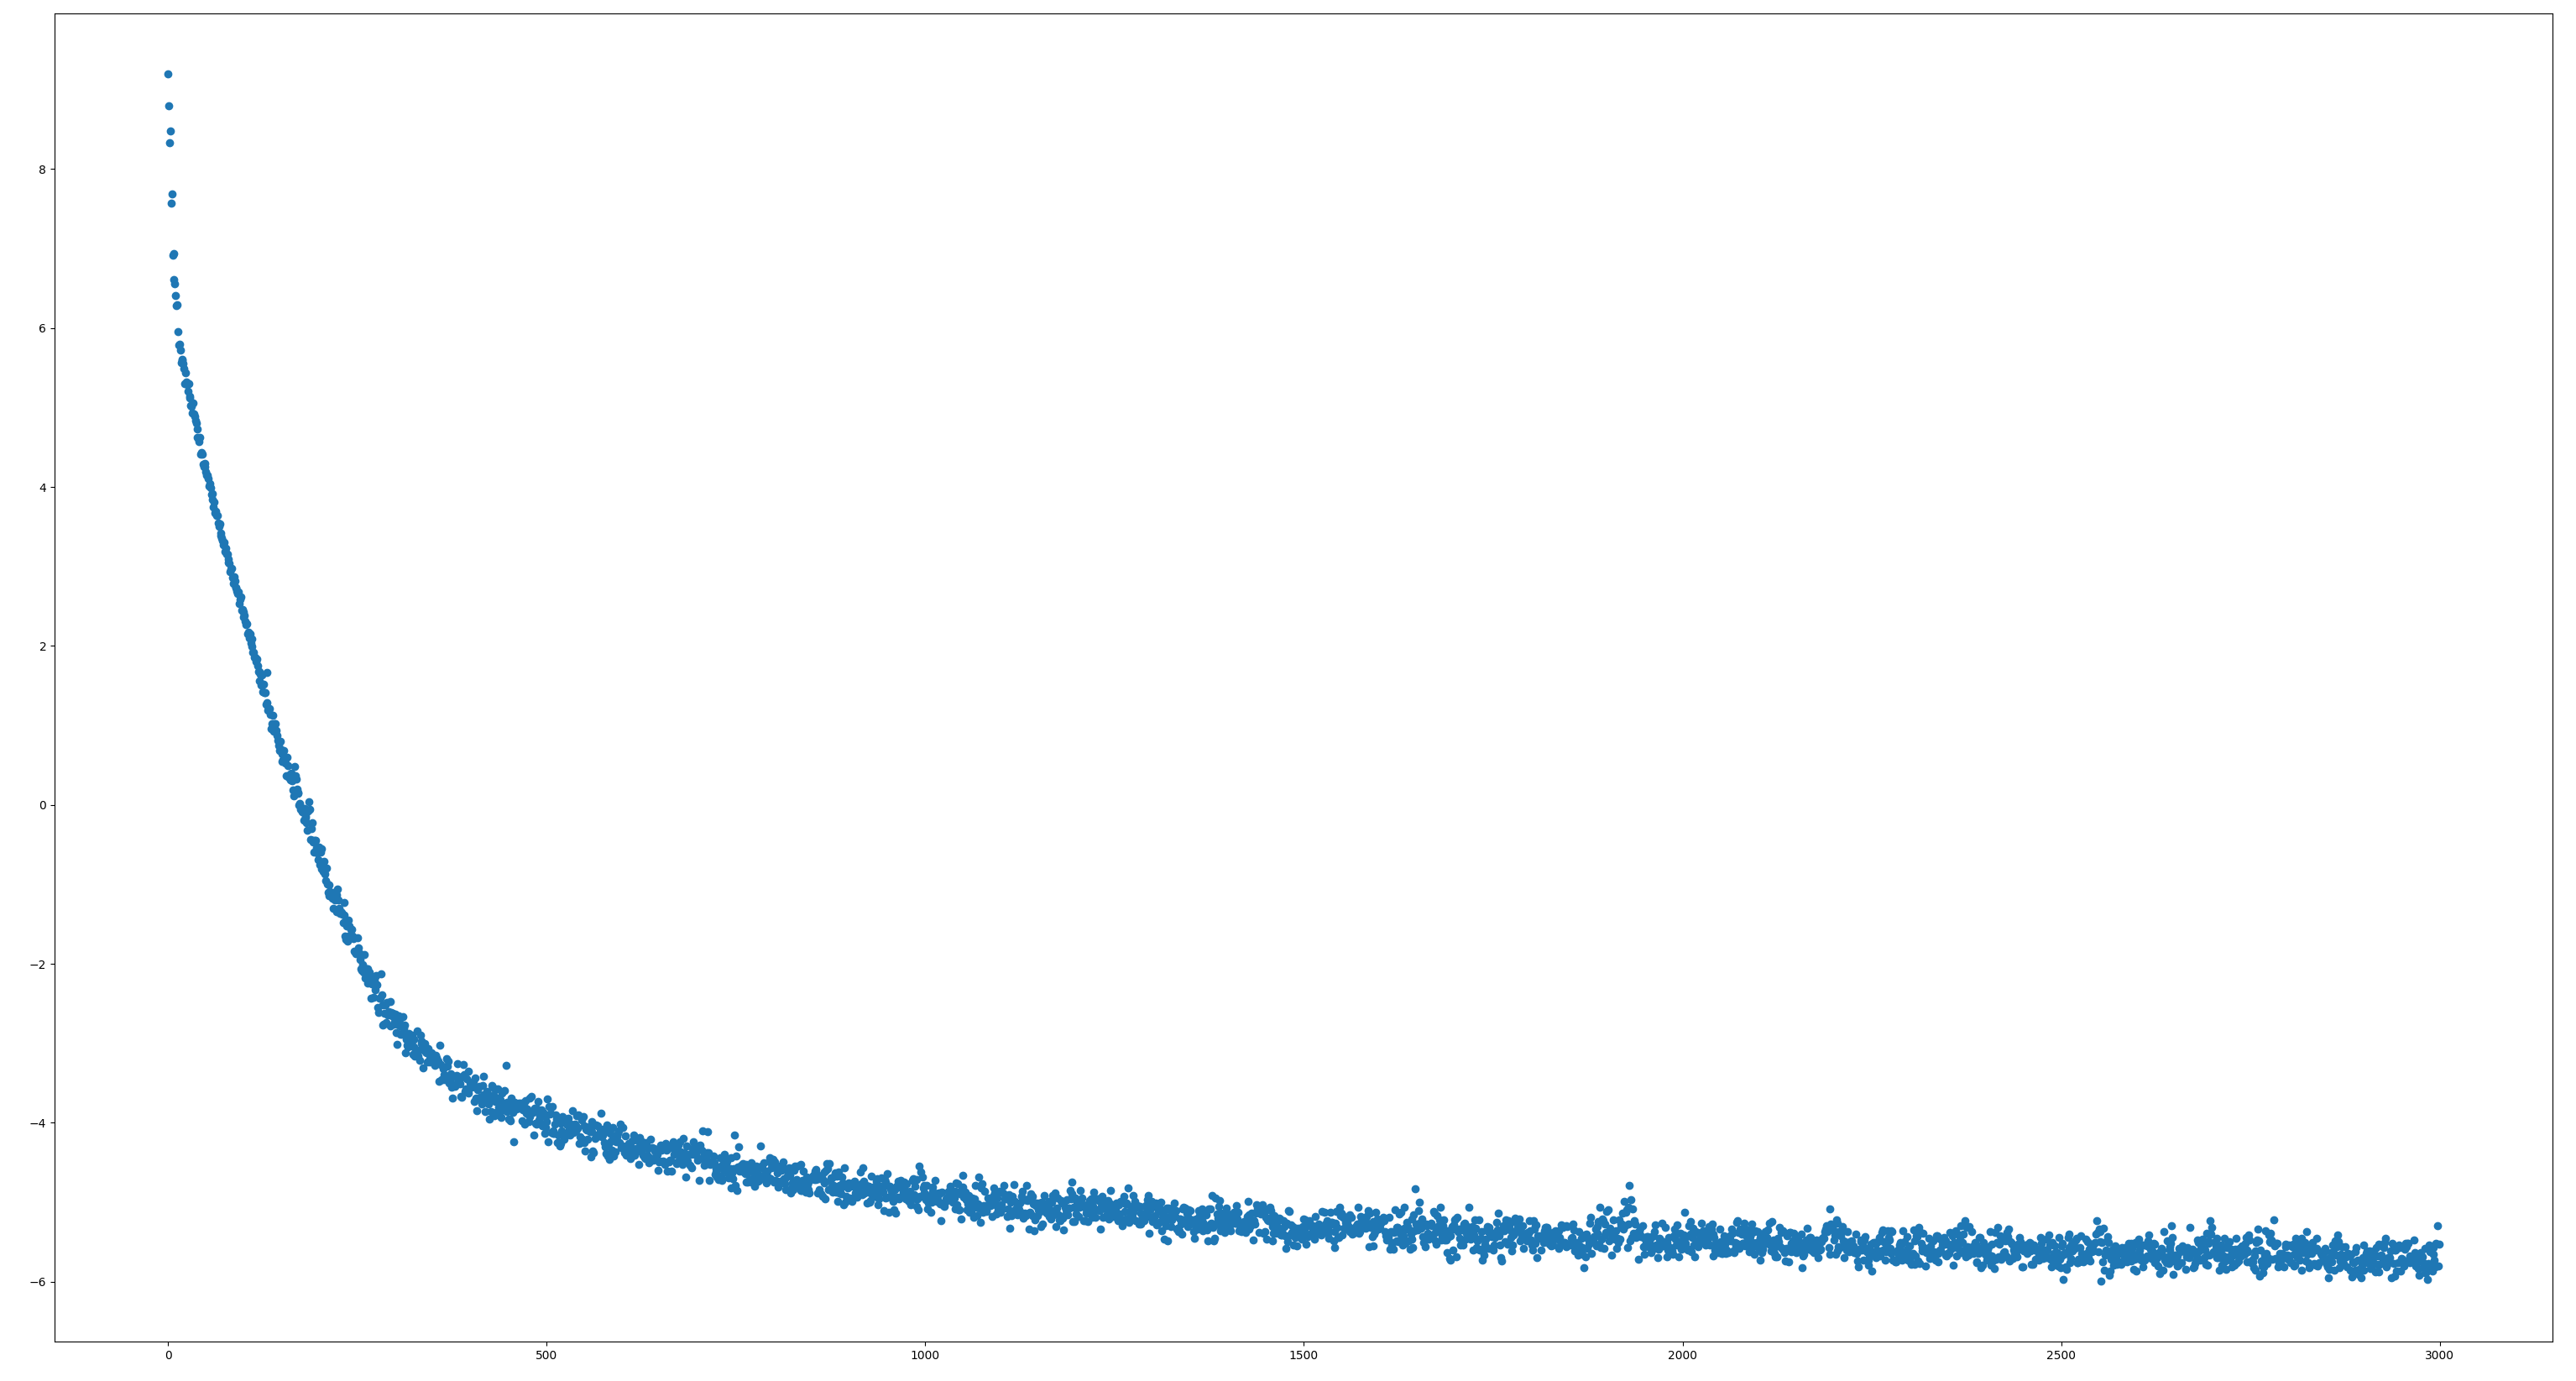
\includegraphics[width = 0.8\textwidth]{Chapters/Ch3-Simulations/normalizing_flows/pics/MeetingFigures/Bobby/LearningRate/learning_rate_25e-5_with_QT.png}
            \caption[Training Loss vs. Epoch]{Epoch (horizontal) vs Training Loss (vertical). Training loss vs. epoch with LR=2.5e-4, using Quantile Transforms. After several hundred epochs, continued training had negligible effect on training loss. }
            \label{fig:jul8_pion_comparison4}
            
        \end{figure}
        


    
    
    \subsubsection{Forward Results from Trained Model}
        Models were trained on 4-feature and 16-feature datasets using conditional normalizing flows, as well as non-conditional flows. \figref{fig:electron_xy_comp} shows a sample result comparing the best performing 16-feature model and the non-conditional model to the traditional simulation distribution. The non-conditional modeling was unable to learn the sharp intricacies of the detector and physics system. The 16-feature conditional MAF model performed well across distributions, but this comes at the cost of requiring conditional input data.  Further sample distributions as comparisons for the 16-feature conditional MAF are displayed in \figref{fig:2D}. 

        \begin{figure}[H]
            \centering
             \begin{minipage}{0.31323\textwidth}
                \centering
                Traditional Simulation
                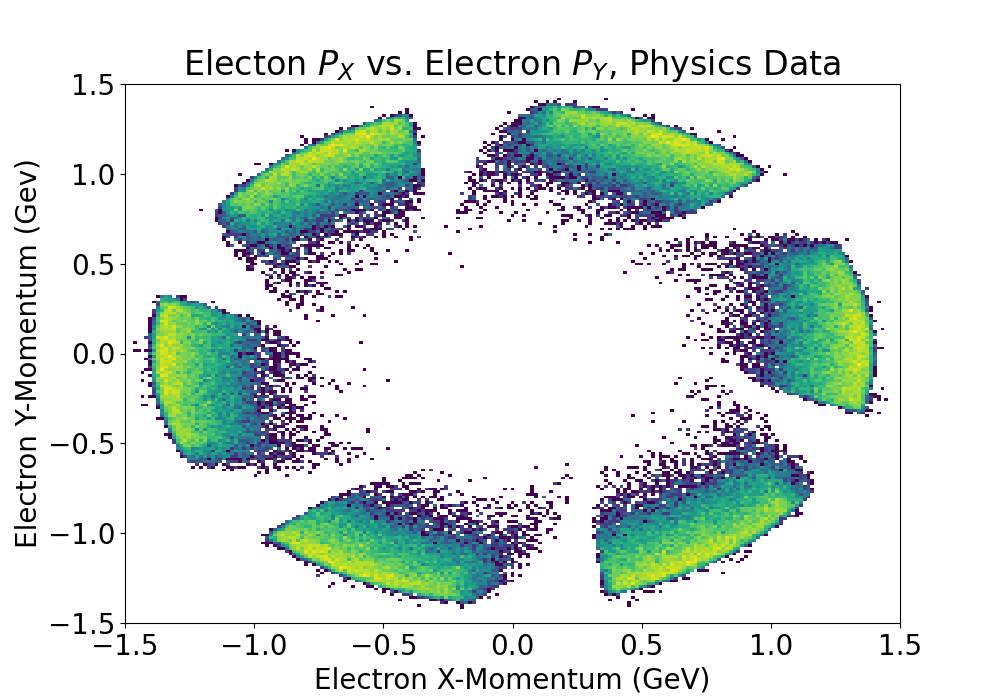
\includegraphics[width=.99\textwidth,trim={0 0 0 0},clip]{Chapters/Ch3-Simulations/normalizing_flows/pics/FinalPictures/Hists2D/Electon_P_X_vs_Electron_P_Y,_Physics_Data.png}
                
            \end{minipage}
                 \begin{minipage}{0.31323\textwidth}
                \centering
                16-Feature Model
                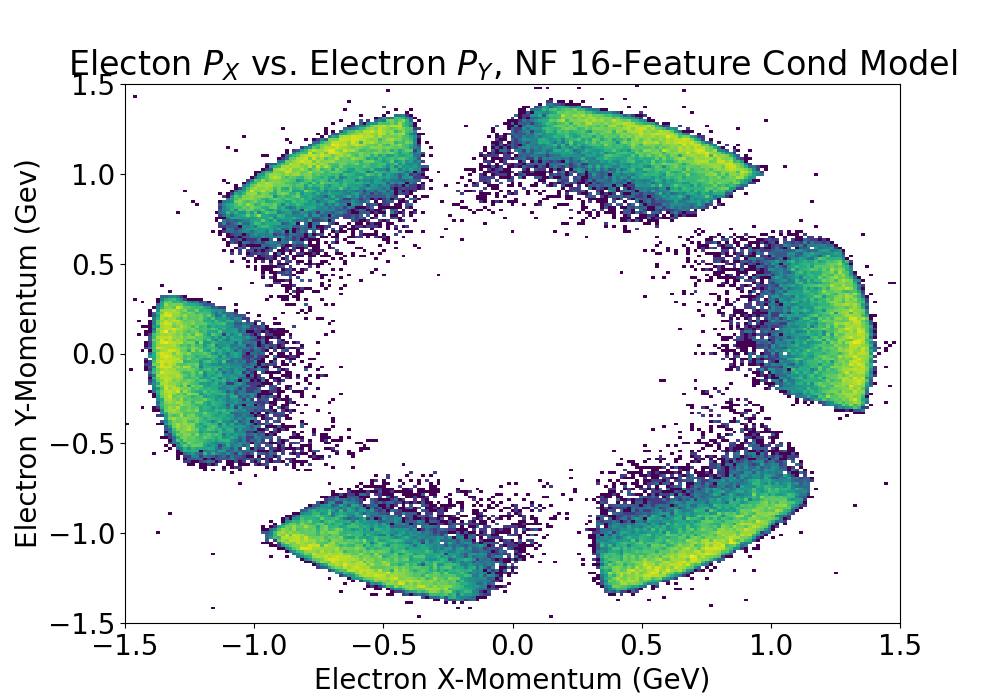
\includegraphics[width=.99\textwidth,trim={0 0 0 0},clip]{Chapters/Ch3-Simulations/normalizing_flows/pics/FinalPictures/Hists2D/Electon_P_X_vs_Electron_P_Y,_NF_16-Feature_Cond_Model.png}
        
            \end{minipage}
                 \begin{minipage}{0.31323\textwidth}
                \centering
                Non-Conditional Model

                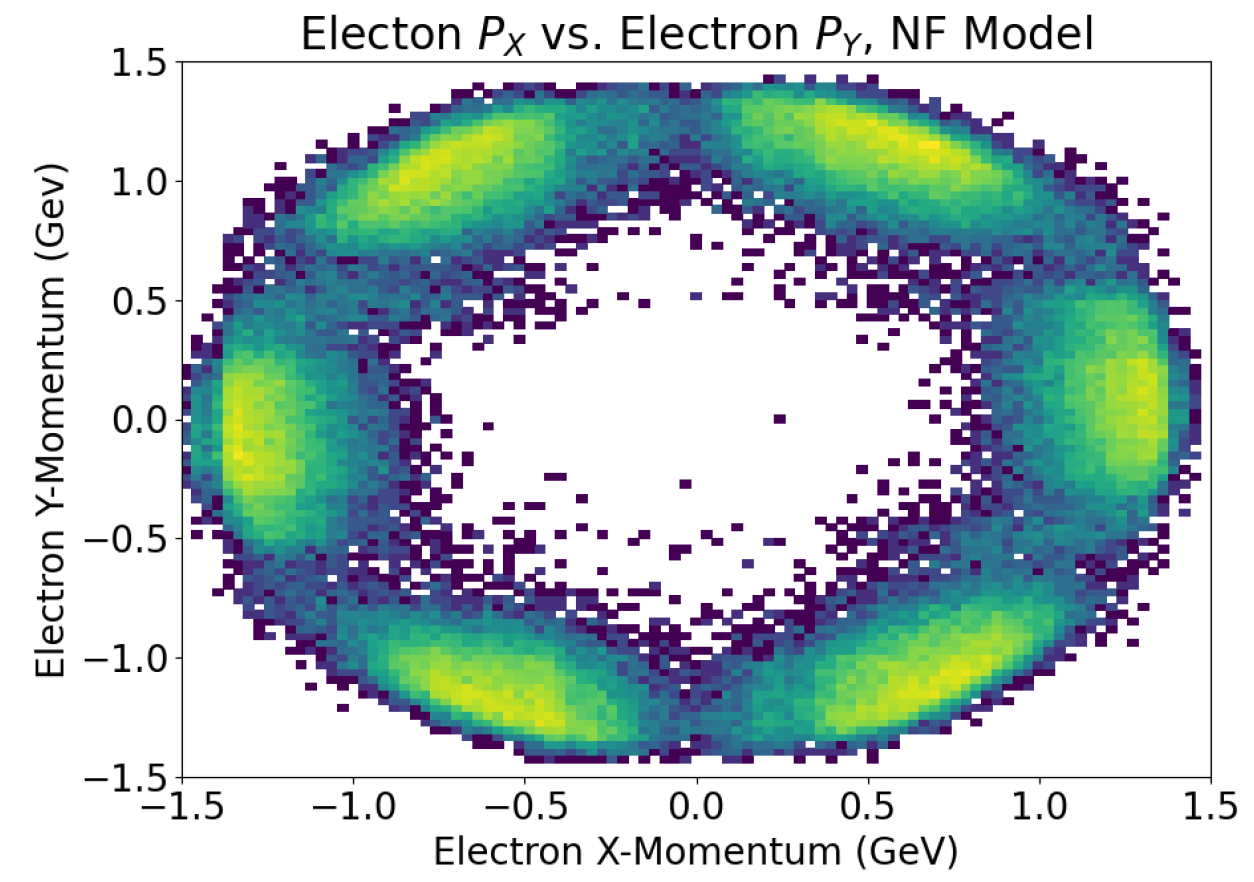
\includegraphics[width=.99\textwidth,trim={0 0 0 0},clip]{Chapters/Ch3-Simulations/normalizing_flows/nonconditional.png}
            \end{minipage}
            \caption[Conditional and Non-conditional Responses]{\textbf{Left}: Electron X-Momentum vs. Electron Y-Momentum distribution from the traditional physics simulation dataset. \textbf{Center}: The observed distribution from the conditional 16-Feature trained model. \textbf{Right}: The distribution result from the non-conditional model, which was unable to learn the sharp detector cutoffs and conservation laws by itself.}
            \label{fig:electron_xy_comp}
        \end{figure}


        \begin{figure}[H]
            \centering
            \begin{minipage}{.3133\textwidth}
            
                \centering
               % Electron
                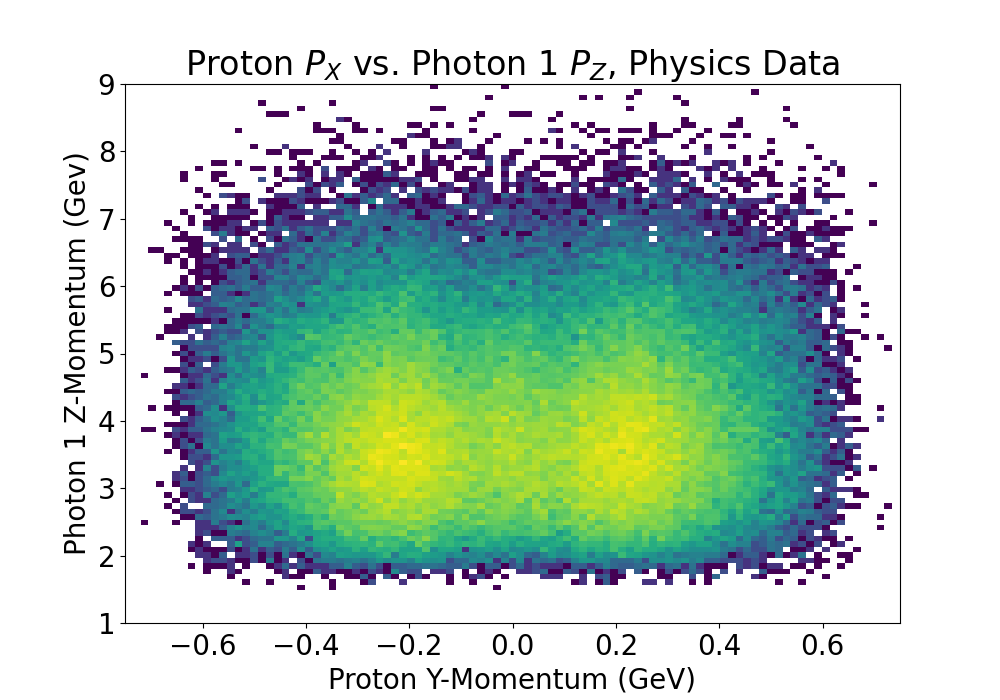
\includegraphics[width=.99\textwidth,trim={0 0 0 0},clip]{Chapters/Ch3-Simulations/normalizing_flows/pics/FinalPictures/Hists2D/Proton_P_X_vs_Photon_1_P_Z,_Physics_Data.png}
                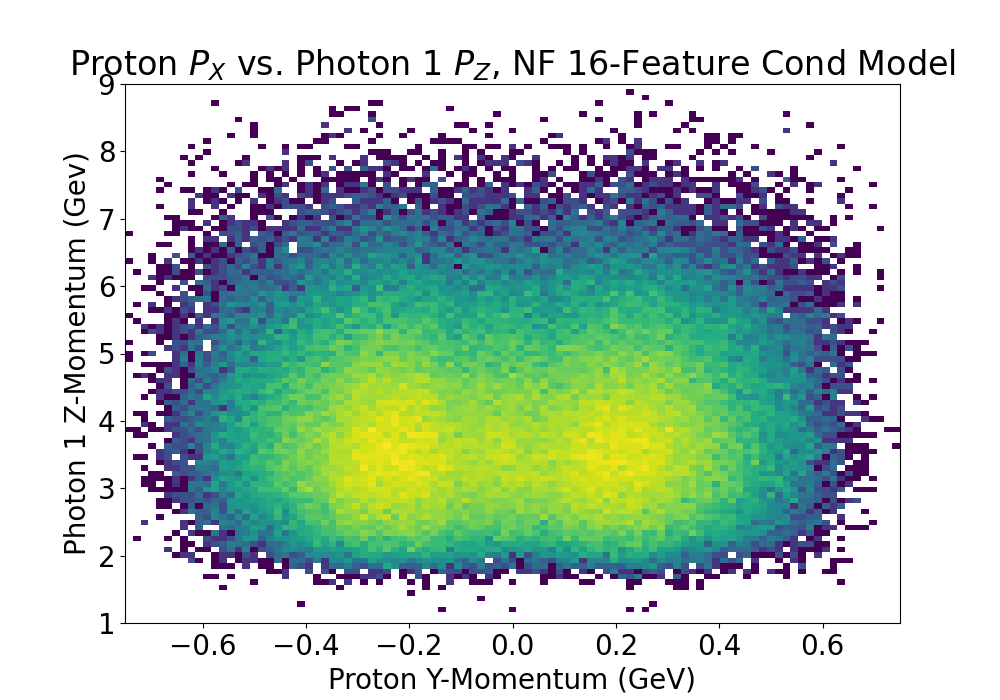
\includegraphics[width=.99\textwidth,trim={0 0 0 0},clip]{Chapters/Ch3-Simulations/normalizing_flows/pics/FinalPictures/Hists2D/Proton_P_X_vs_Photon_1_P_Z,_NF_16-Feature_Cond_Model.png}
        
            \end{minipage}%
            \begin{minipage}{0.3133\textwidth}
                \centering
               %Feature Distributions from Traditional Microphysics Simulations
                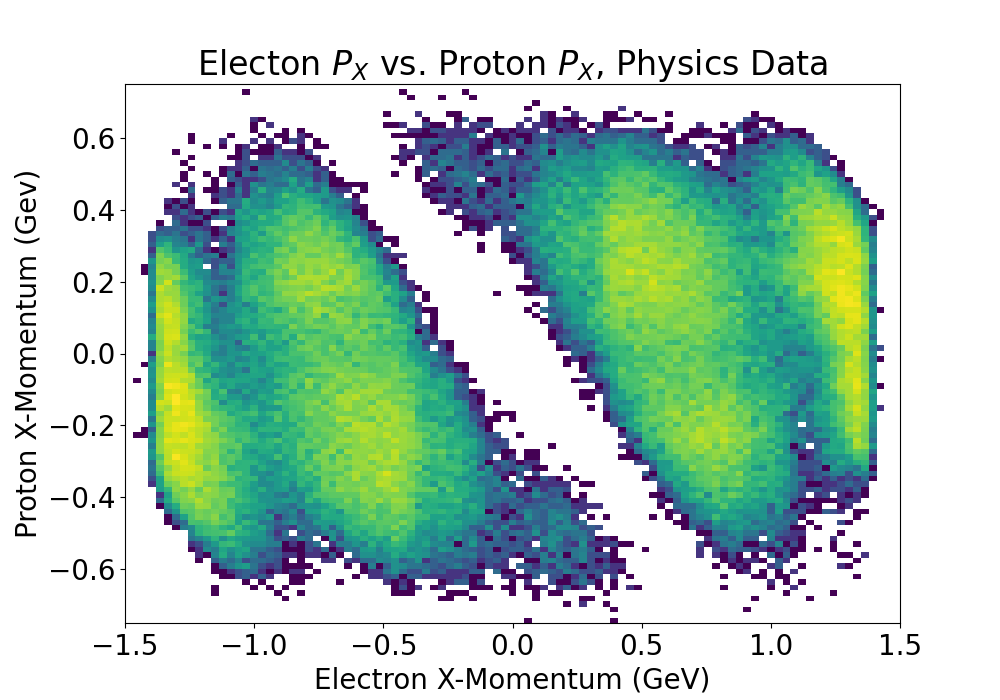
\includegraphics[width=.99\textwidth,trim={0 0 0 0},clip]{Chapters/Ch3-Simulations/normalizing_flows/pics/FinalPictures/Hists2D/Electon_P_X_vs_Proton_P_X,_Physics_Data.png}
                %Feature Distributions from NF Model Samples
                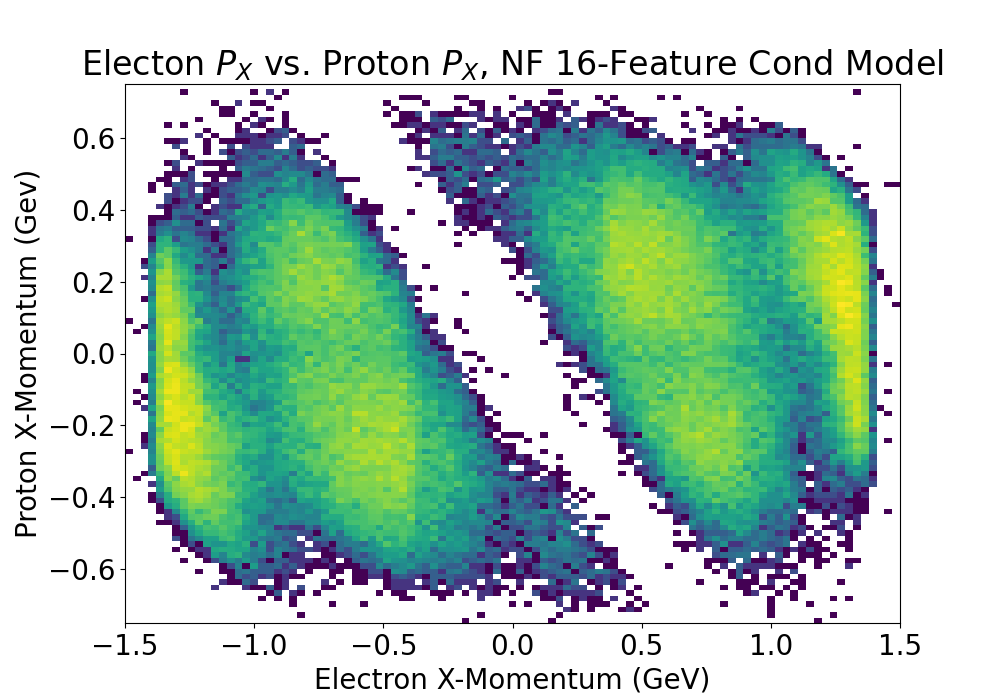
\includegraphics[width=.99\textwidth,trim={0 0 0 0},clip]{Chapters/Ch3-Simulations/normalizing_flows/pics/FinalPictures/Hists2D/Electon_P_X_vs_Proton_P_X,_NF_16-Feature_Cond_Model.png}
                
        
            \end{minipage}
             \begin{minipage}{0.3133\textwidth}
                    \centering
                   % Photon 1
                    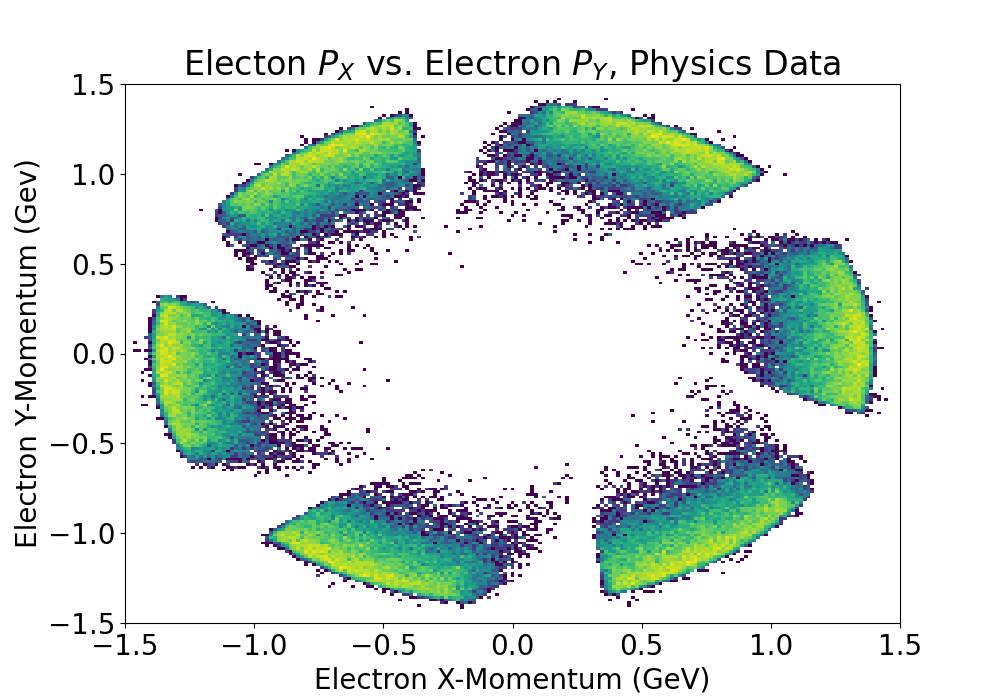
\includegraphics[width=.99\textwidth,trim={0 0 0 0},clip]{Chapters/Ch3-Simulations/normalizing_flows/pics/FinalPictures/Hists2D/Electon_P_X_vs_Electron_P_Y,_Physics_Data.png}
                    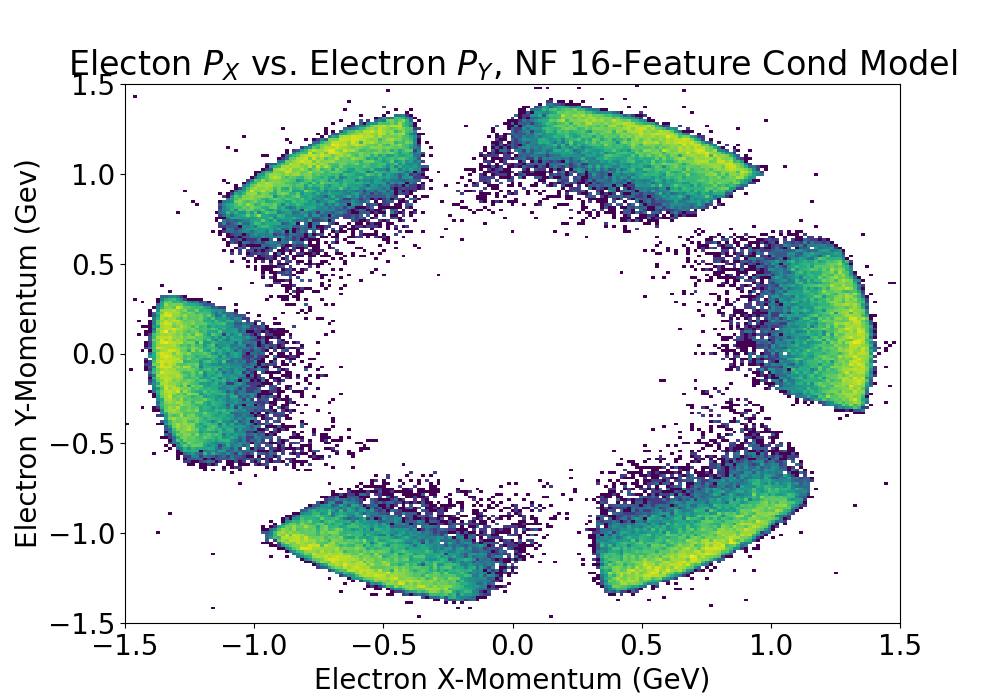
\includegraphics[width=.99\textwidth,trim={0 0 0 0},clip]{Chapters/Ch3-Simulations/normalizing_flows/pics/FinalPictures/Hists2D/Electon_P_X_vs_Electron_P_Y,_NF_16-Feature_Cond_Model.png}
        
            \end{minipage}
            \caption[16-feature Result Sample Distributions]{ 2-Dimensional distributions for various features, comparing the data from the traditional physics simulation to the NF sampled data. \textbf{Top} Feature distributions from the traditional physics data set. \textbf{Bottom} Feature distributions from our trained NF model, which should match with the top row. Moving from left to right, we can see that some feature distributions are reproduced well, while others have difficult details that are not well modeled, corresponding to physical detector geometry and physics constraints that the NF model is unaware of. }
            \label{fig:2D}
        \end{figure}
        
        Figure \ref{fig:16features} shows all 16 feature distributions of samples from this trained model, with each plot also showing the Earth Mover's Distance between the NF model data, and sample data from the microphysics distribution. Good agreement is found for all features, although the proton seems to perform slightly worse than the other particles. 

        \begin{figure}[H]
            \centering
            \begin{minipage}{.23\textwidth}
            
                \centering
               % Electron
                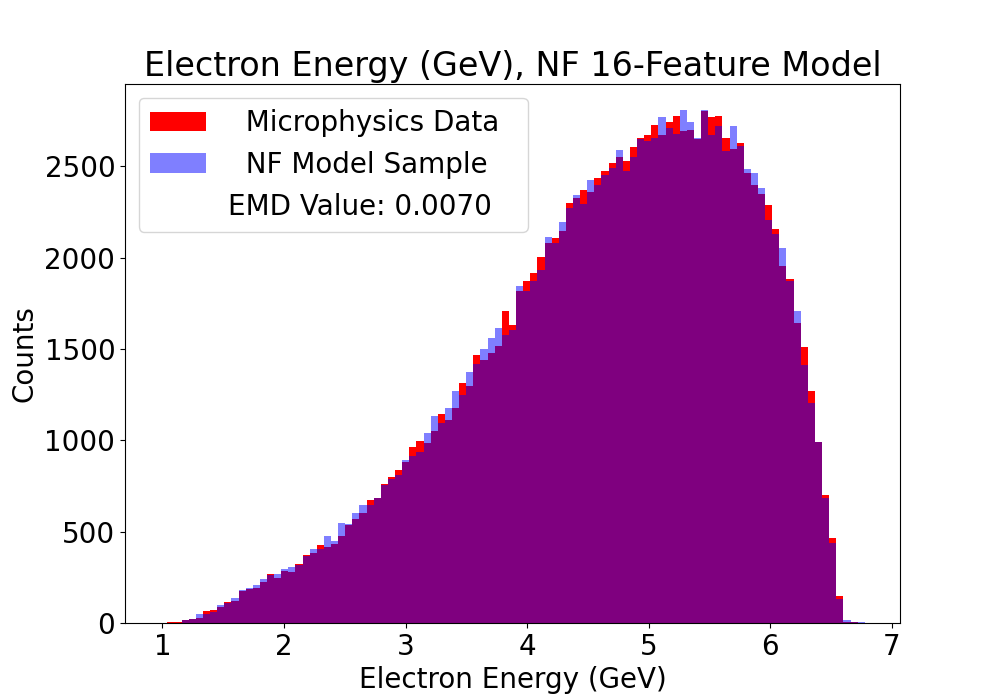
\includegraphics[width=.99\textwidth,trim={3cm 0 0 0},clip]{Chapters/Ch3-Simulations/normalizing_flows/pics/FinalPictures/Features16/Electron_Energy_,_NF_16-Feature_Model.png}
                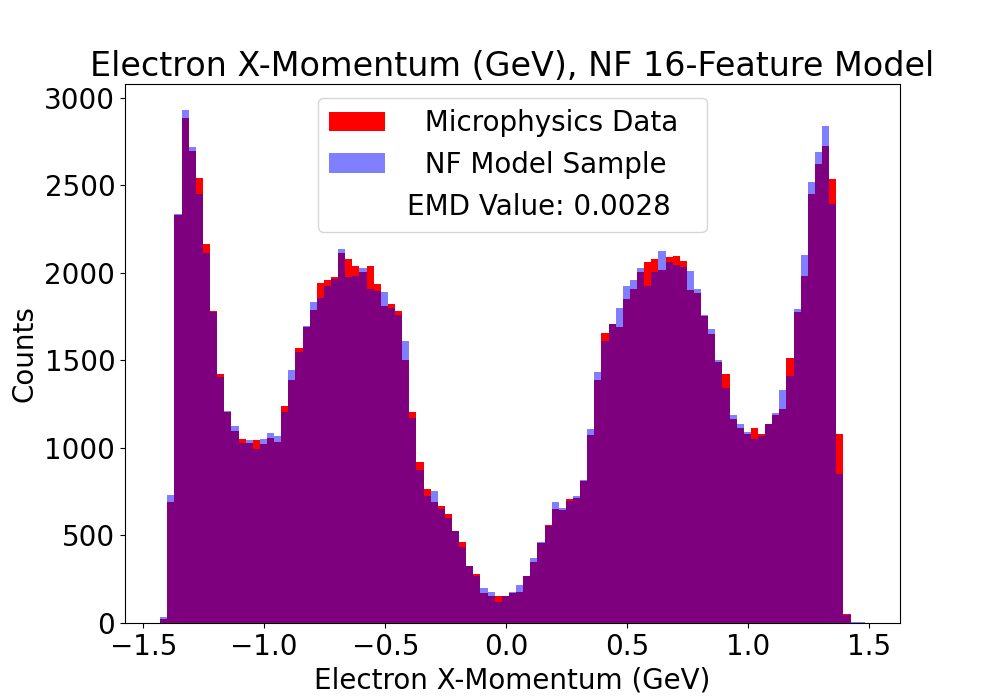
\includegraphics[width=.99\textwidth,trim={3cm 0 0 0},clip]{Chapters/Ch3-Simulations/normalizing_flows/pics/FinalPictures/Features16/Electron_X-Momentum_,_NF_16-Feature_Model.png}
                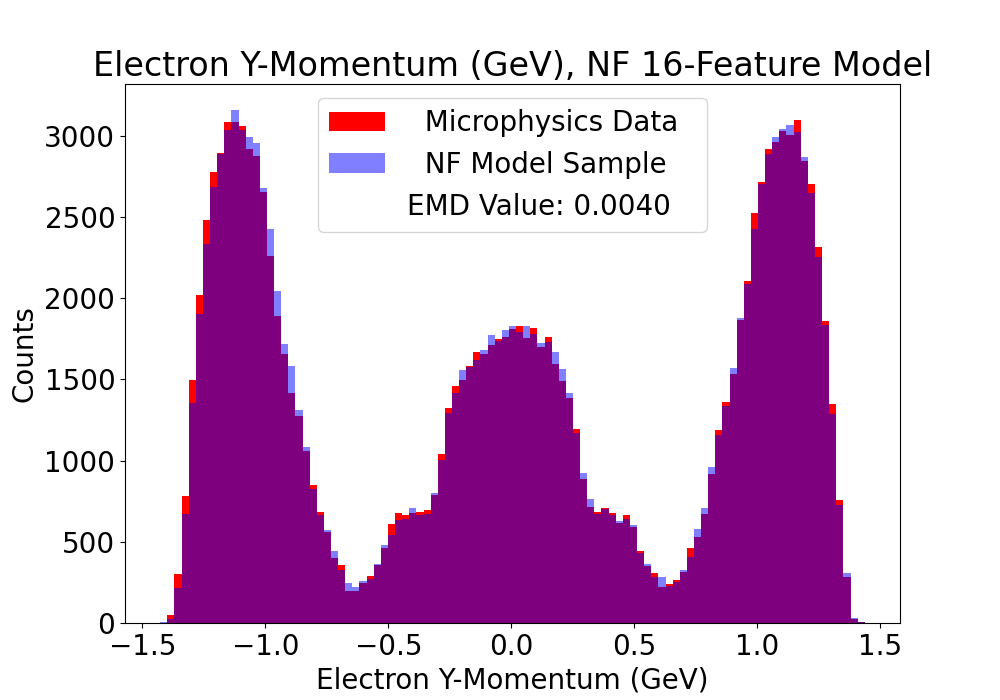
\includegraphics[width=.99\textwidth,trim={3cm 0 0 0},clip]{Chapters/Ch3-Simulations/normalizing_flows/pics/FinalPictures/Features16/Electron_Y-Momentum_,_NF_16-Feature_Model.png}
                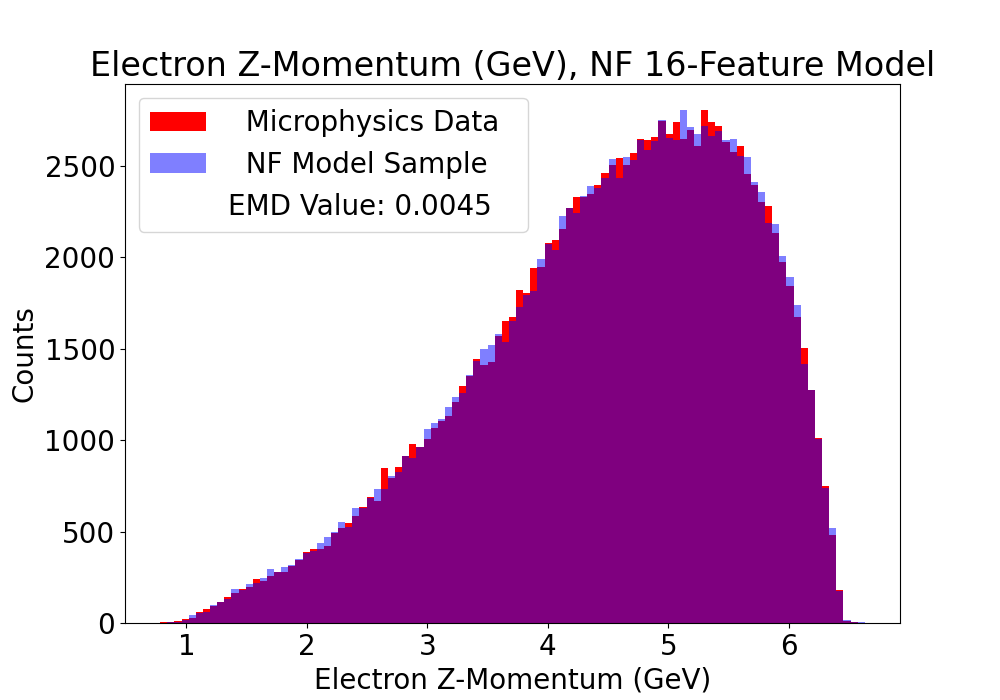
\includegraphics[width=.99\textwidth,trim={3cm 0 0 0},clip]{Chapters/Ch3-Simulations/normalizing_flows/pics/FinalPictures/Features16/Electron_Z-Momentum_,_NF_16-Feature_Model.png}
            \end{minipage}%
            \begin{minipage}{0.23\textwidth}
                \centering
               % Proton
                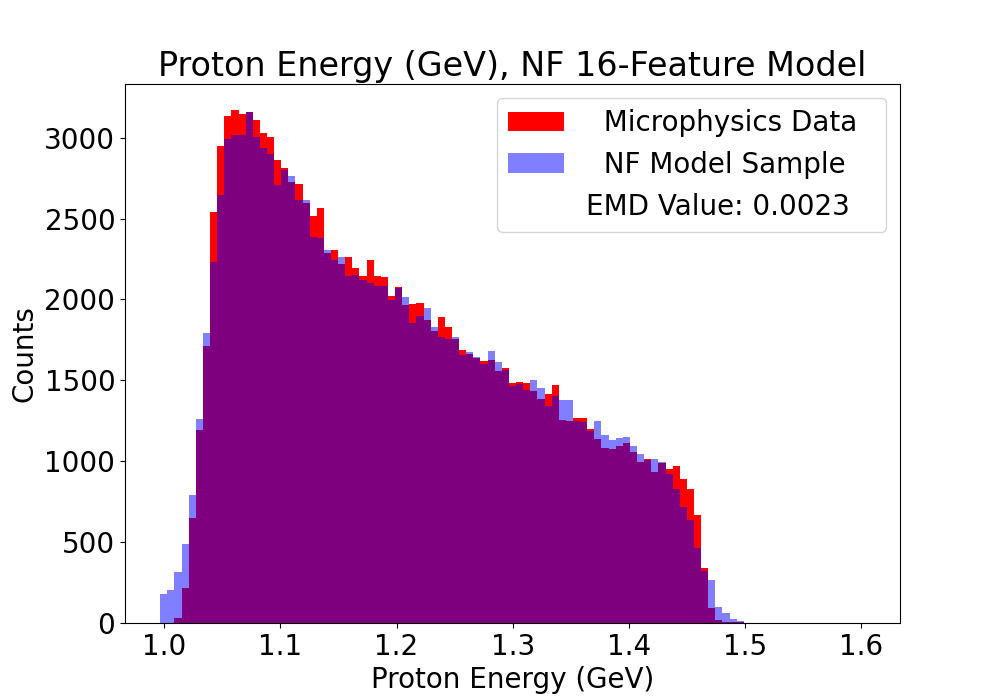
\includegraphics[width=.99\textwidth,trim={3cm 0 0 0},clip]{Chapters/Ch3-Simulations/normalizing_flows/pics/FinalPictures/Features16/Proton_Energy_,_NF_16-Feature_Model.png}
                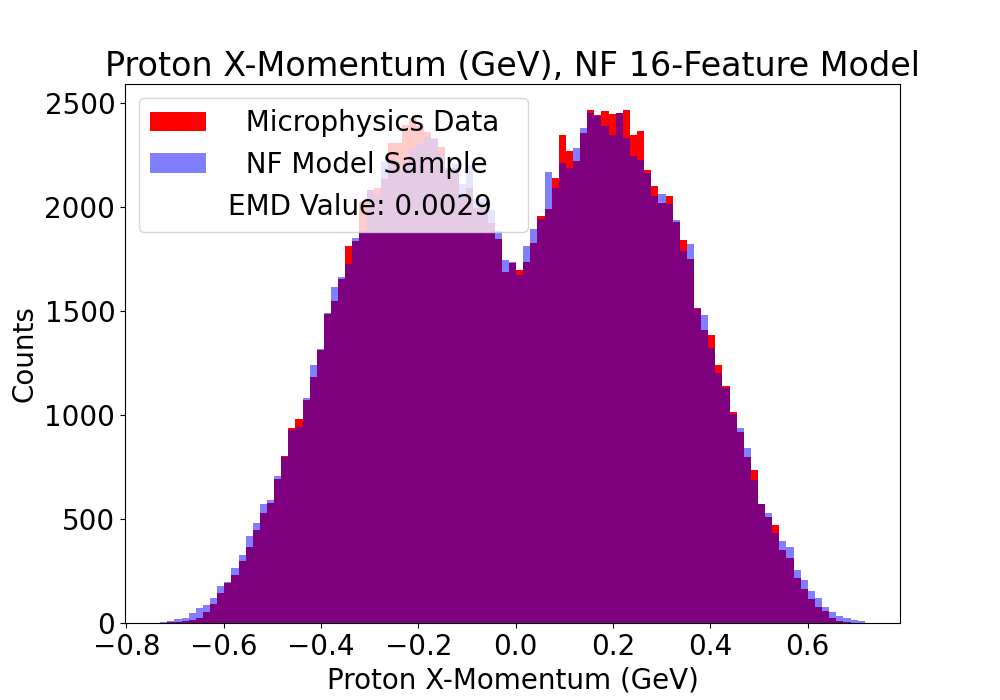
\includegraphics[width=.99\textwidth,trim={3cm 0 0 0},clip]{Chapters/Ch3-Simulations/normalizing_flows/pics/FinalPictures/Features16/Proton_X-Momentum_,_NF_16-Feature_Model.png}
                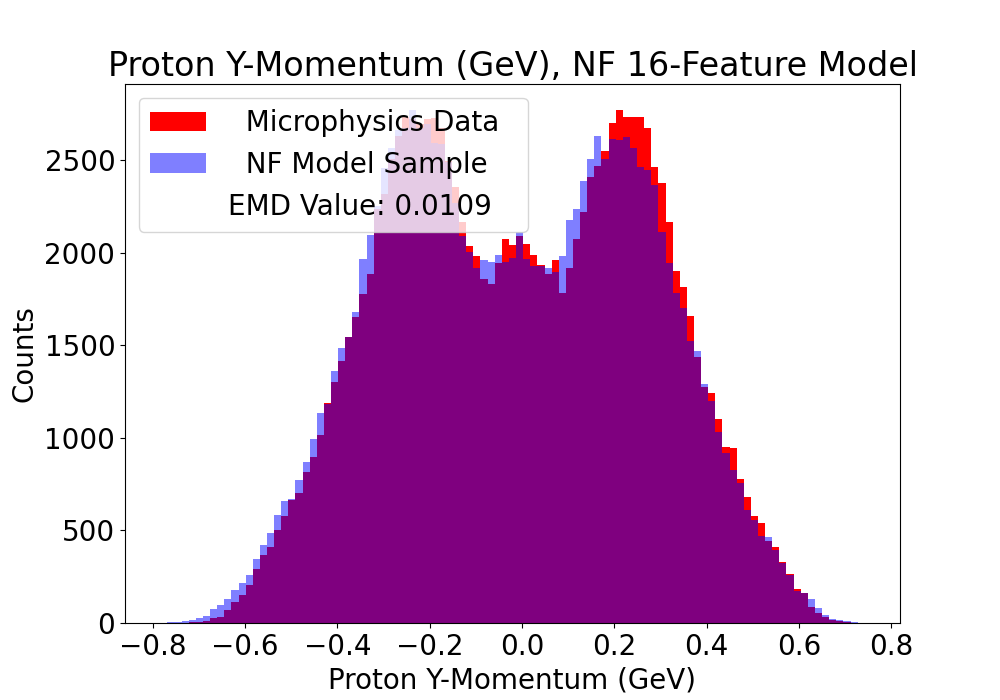
\includegraphics[width=.99\textwidth,trim={3cm 0 0 0},clip]{Chapters/Ch3-Simulations/normalizing_flows/pics/FinalPictures/Features16/Proton_Y-Momentum_,_NF_16-Feature_Model.png}
                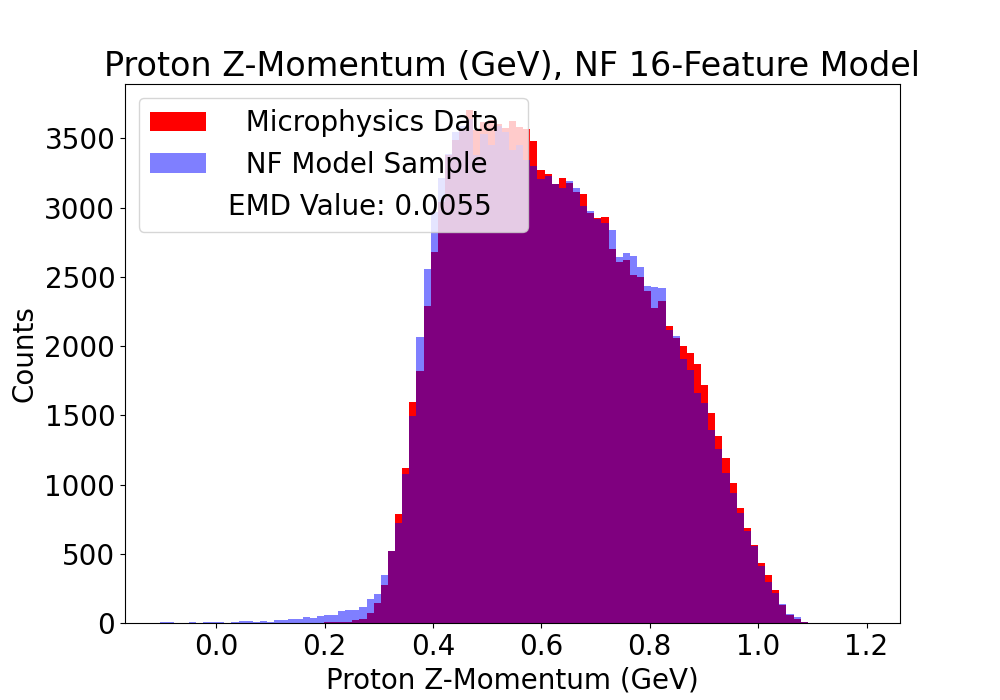
\includegraphics[width=.99\textwidth,trim={3cm 0 0 0},clip]{Chapters/Ch3-Simulations/normalizing_flows/pics/FinalPictures/Features16/Proton_Z-Momentum_,_NF_16-Feature_Model.png}
            \end{minipage}
             \begin{minipage}{0.23\textwidth}
                    \centering
                   % Photon 1
                    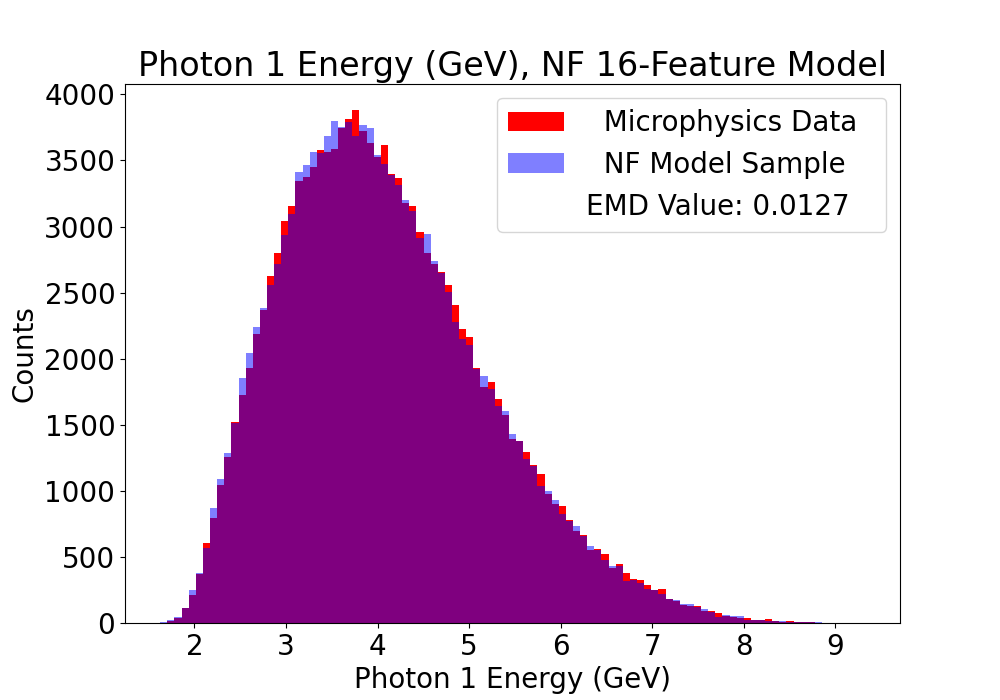
\includegraphics[width=.99\textwidth,trim={3cm 0 0 0},clip]{Chapters/Ch3-Simulations/normalizing_flows/pics/FinalPictures/Features16/Photon_1_Energy_,_NF_16-Feature_Model.png}
                    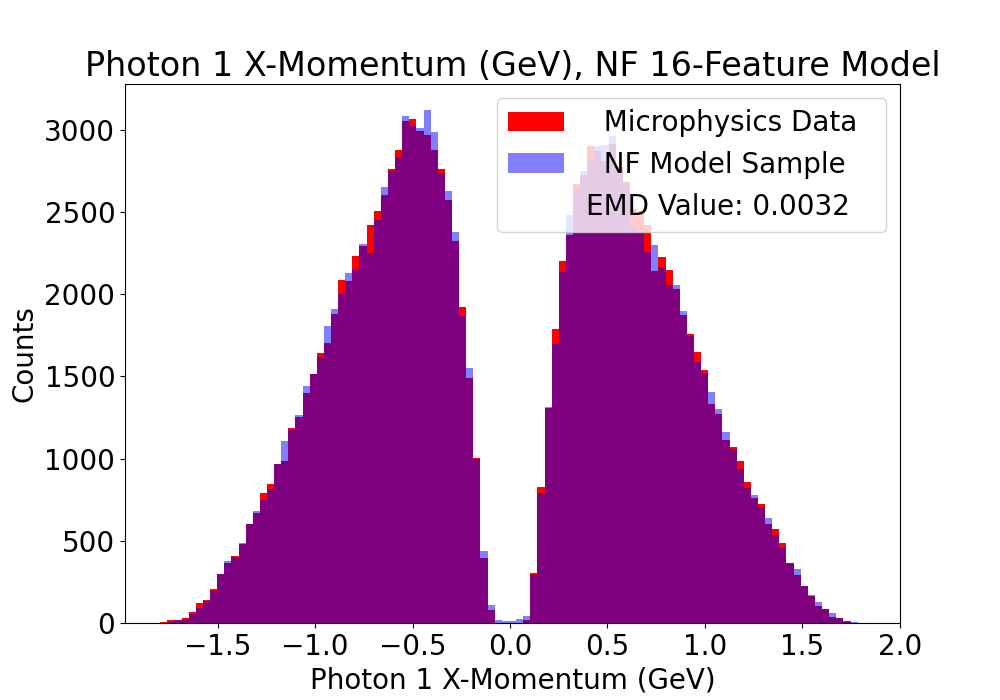
\includegraphics[width=.99\textwidth,trim={3cm 0 0 0},clip]{Chapters/Ch3-Simulations/normalizing_flows/pics/FinalPictures/Features16/Photon_1_X-Momentum_,_NF_16-Feature_Model.png}
                    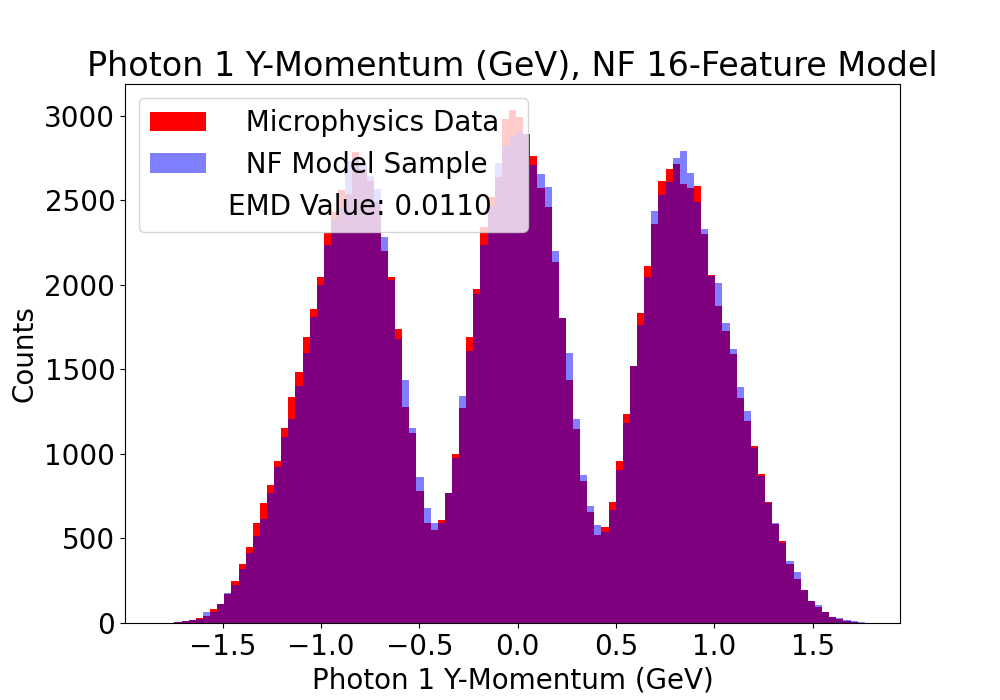
\includegraphics[width=.99\textwidth,trim={3cm 0 0 0},clip]{Chapters/Ch3-Simulations/normalizing_flows/pics/FinalPictures/Features16/Photon_1_Y-Momentum_,_NF_16-Feature_Model.png}
                    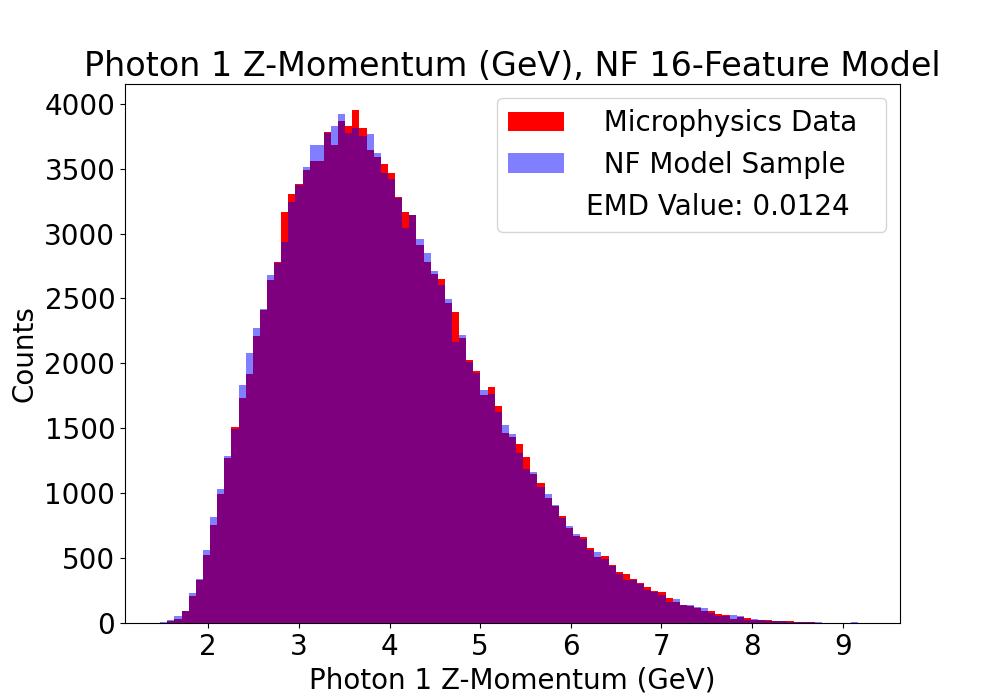
\includegraphics[width=.99\textwidth,trim={3cm 0 0 0},clip]{Chapters/Ch3-Simulations/normalizing_flows/pics/FinalPictures/Features16/Photon_1_Z-Momentum_,_NF_16-Feature_Model.png}
            \end{minipage}
             \begin{minipage}{0.23\textwidth}
                \centering
                %Photon 2
                
                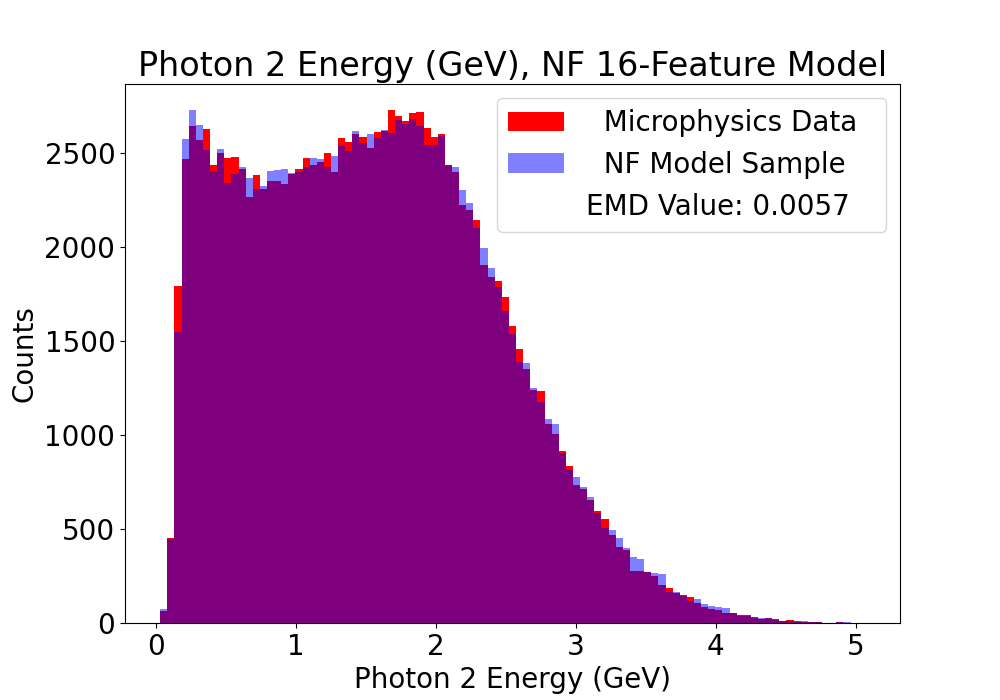
\includegraphics[width=.99\textwidth,trim={3cm 0 0 0},clip]{Chapters/Ch3-Simulations/normalizing_flows/pics/FinalPictures/Features16/Photon_2_Energy_,_NF_16-Feature_Model.png}
                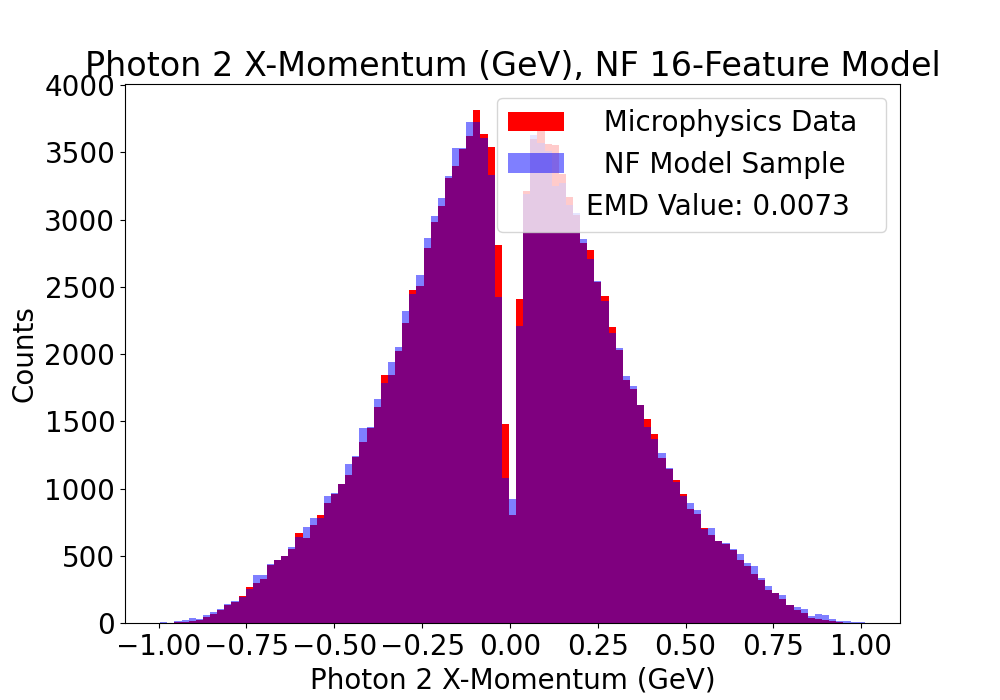
\includegraphics[width=.99\textwidth,trim={3cm 0 0 0},clip]{Chapters/Ch3-Simulations/normalizing_flows/pics/FinalPictures/Features16/Photon_2_X-Momentum_,_NF_16-Feature_Model.png}
                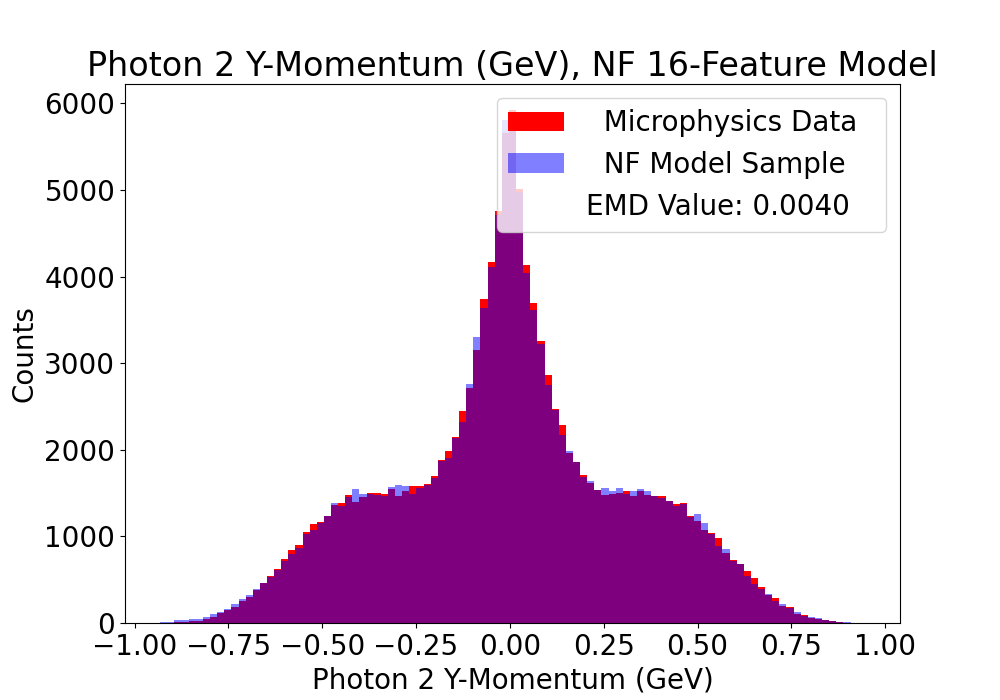
\includegraphics[width=.99\textwidth,trim={3cm 0 0 0},clip]{Chapters/Ch3-Simulations/normalizing_flows/pics/FinalPictures/Features16/Photon_2_Y-Momentum_,_NF_16-Feature_Model.png}
                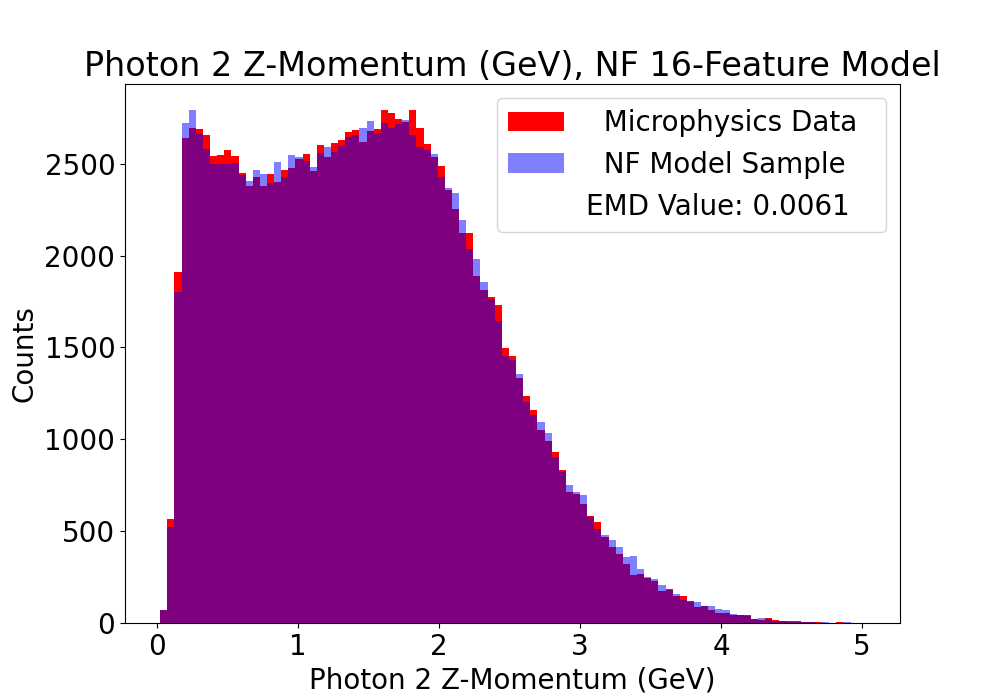
\includegraphics[width=.99\textwidth,trim={3cm 0 0 0},clip]{Chapters/Ch3-Simulations/normalizing_flows/pics/FinalPictures/Features16/Photon_2_Z-Momentum_,_NF_16-Feature_Model.png}
            \end{minipage}
            \caption[1D Distributions of 16 feature Result]{The 1D distributions of all 16 features sampled from our NF model (blue), and from physics simulation (red). Each histogram is normalized to the area, and has 100 bins.}
            \label{fig:16features}
        \end{figure}

        For a quantitative comparison, Figure \ref{fig:EMD} shows the Earth Mover's Distance between samples from the trained NF model and the traditional physics distribution. In the limit of identical distributions with infinitely many samples, the EMD is zero. Since we are working with only 100K datapoints, rather than report the EMD values by themselves (which can be seen in Figure \ref{fig:16features}), we took the ratio of the NF model - traditional physics distribution EMD value to the EMD value calculated between two sets of 100K datapoints taken from the traditional physics distribution, which had values on the order of 0.005. Thus, a perfectly trained NF model would have an EMD ratio of 1, and as we deviate above 1, we exhibit worse performance.  
        

        \begin{figure}[H]
            \centering
            %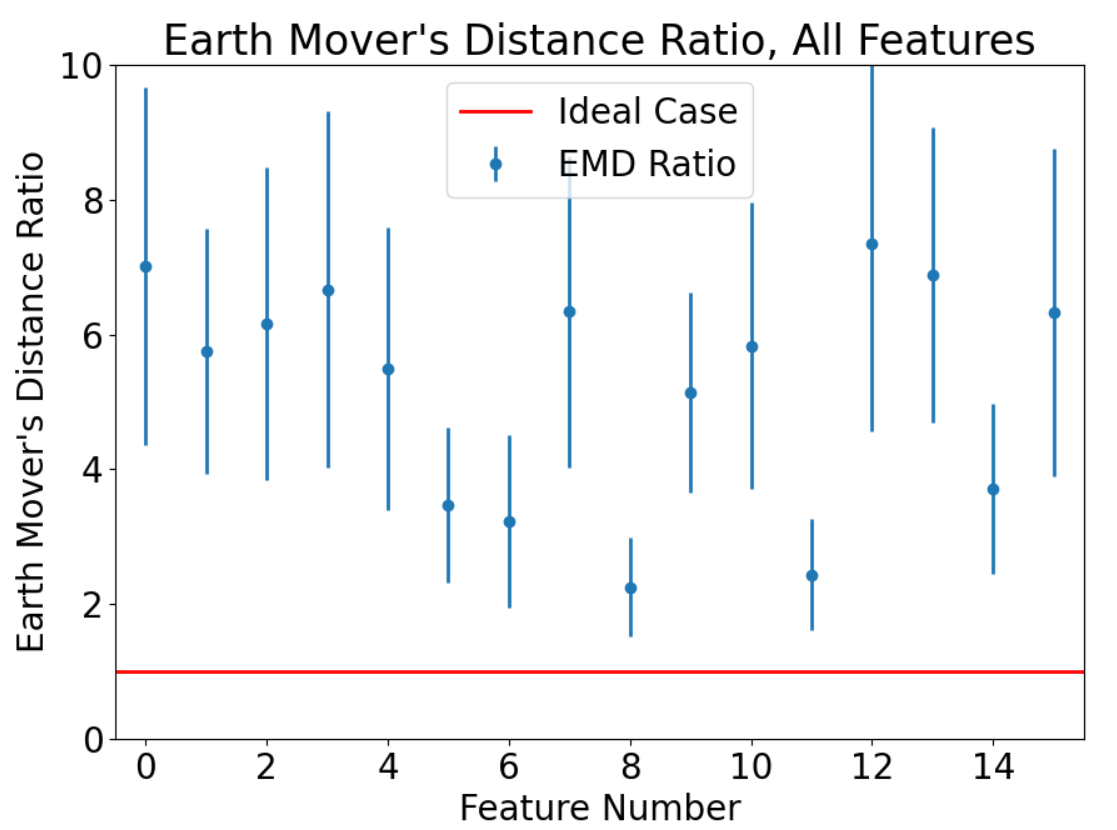
\includegraphics[scale=0.3]{FinalPictures/EMD/EmdRatio.png}
            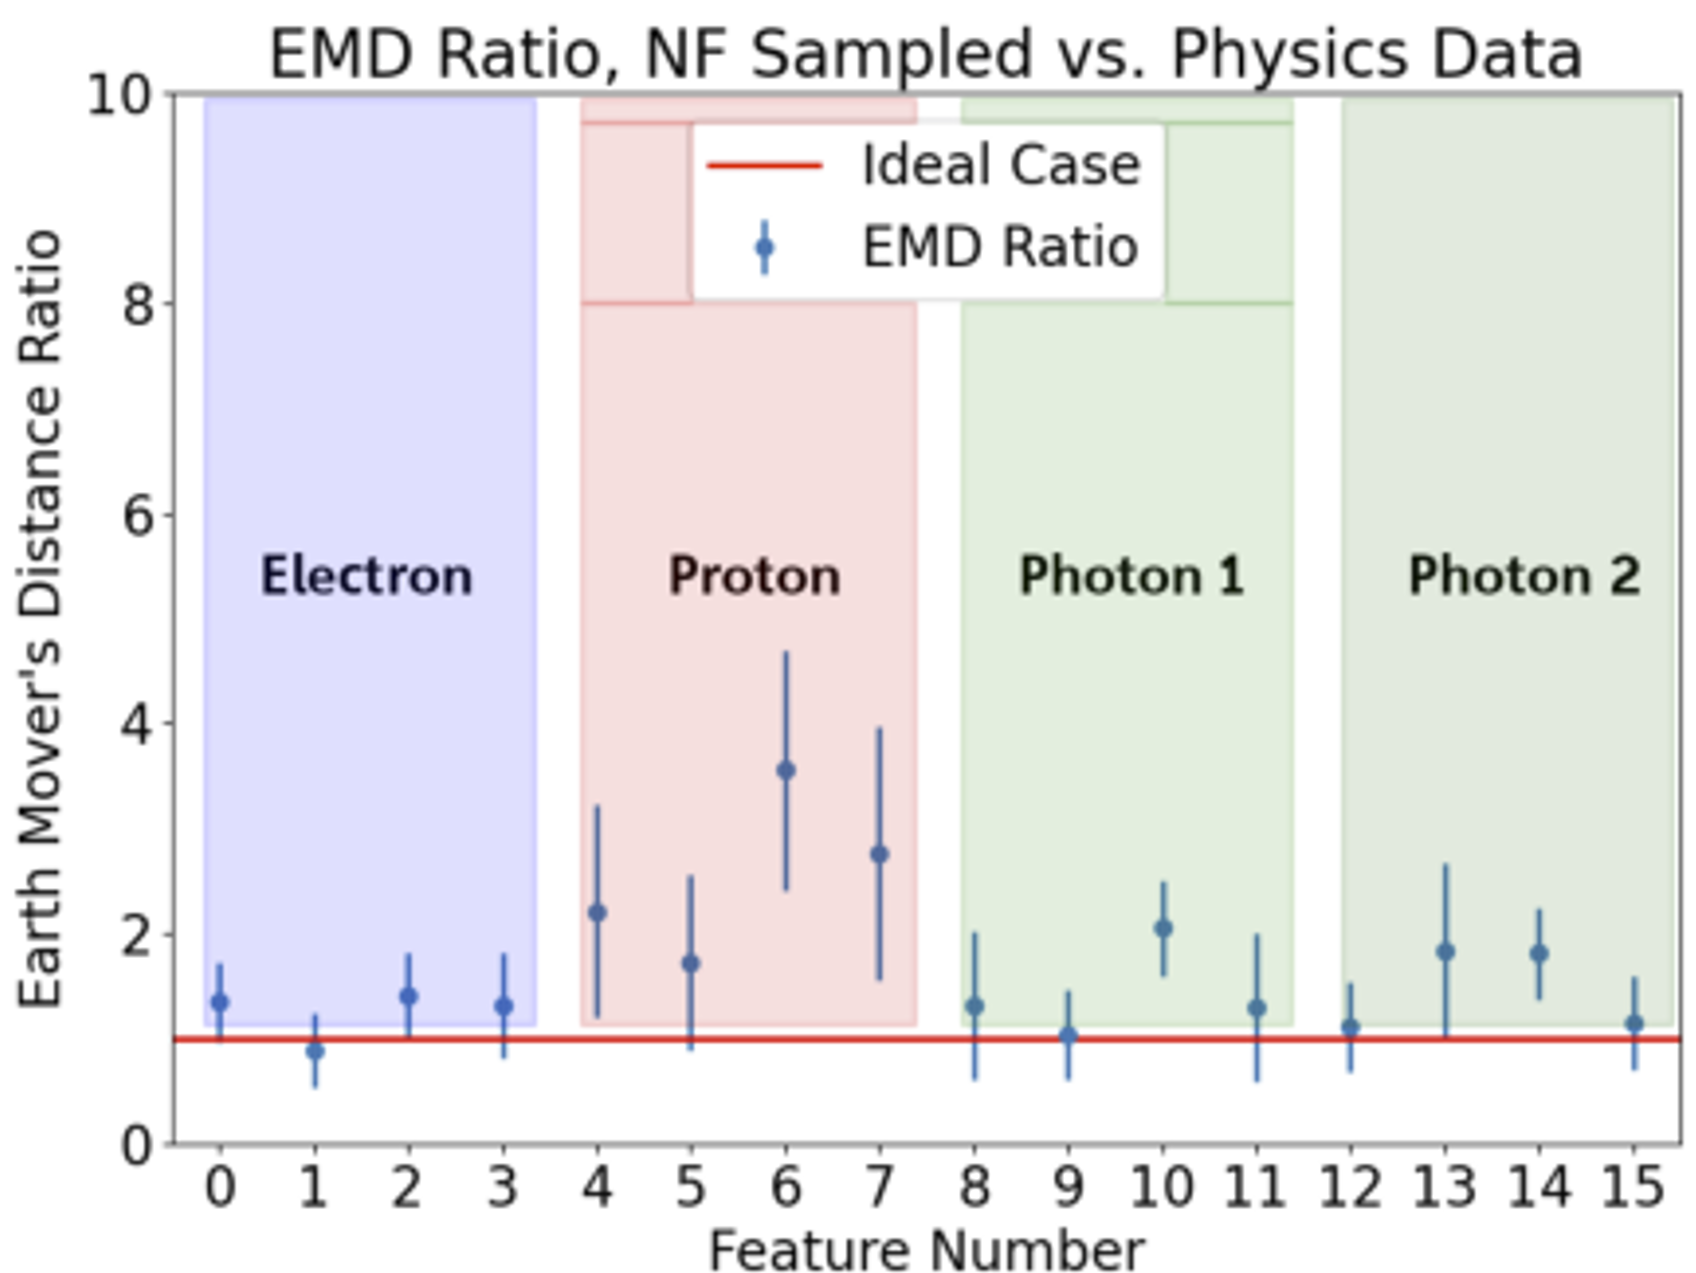
\includegraphics[width=.8\textwidth,trim={0 0 0 0 },clip]{Chapters/Ch3-Simulations/normalizing_flows/pics/FinalPictures/EMD/EMD_updated.png}
            \caption[Earth Mover's Distance Ratio]{The EMD ratios of all 16 features between the 16-feature conditional MAF generated distributions and sample from physics simulation. The points are the average EMD ratios of 10 different subsample calculations; the error bars are the standard deviations of the sets. If the model were perfect, all points would have value 1; deviation from 1 indicates worse performance.}
            \label{fig:EMD}
        \end{figure}
        
    
        Ultimately, we are interested in physics processes rather than just distribution mapping, so we also examined our ability to reconstruct physics quantities from the trained NF model sample data. Figure \ref{fig:protonspions} shows the distribution of calculated proton and pion (calculated from a combination of the photon features) masses from our NF model data, which had no explicit physics constraints in training. We observe a peak at about 0.939 GeV for the proton and 0.136 GeV for the pion, , which is within 0.5\% of the value encapsulated in the traditional physics training dataset. 
        
        
        \begin{figure}[H]
            \centering
            %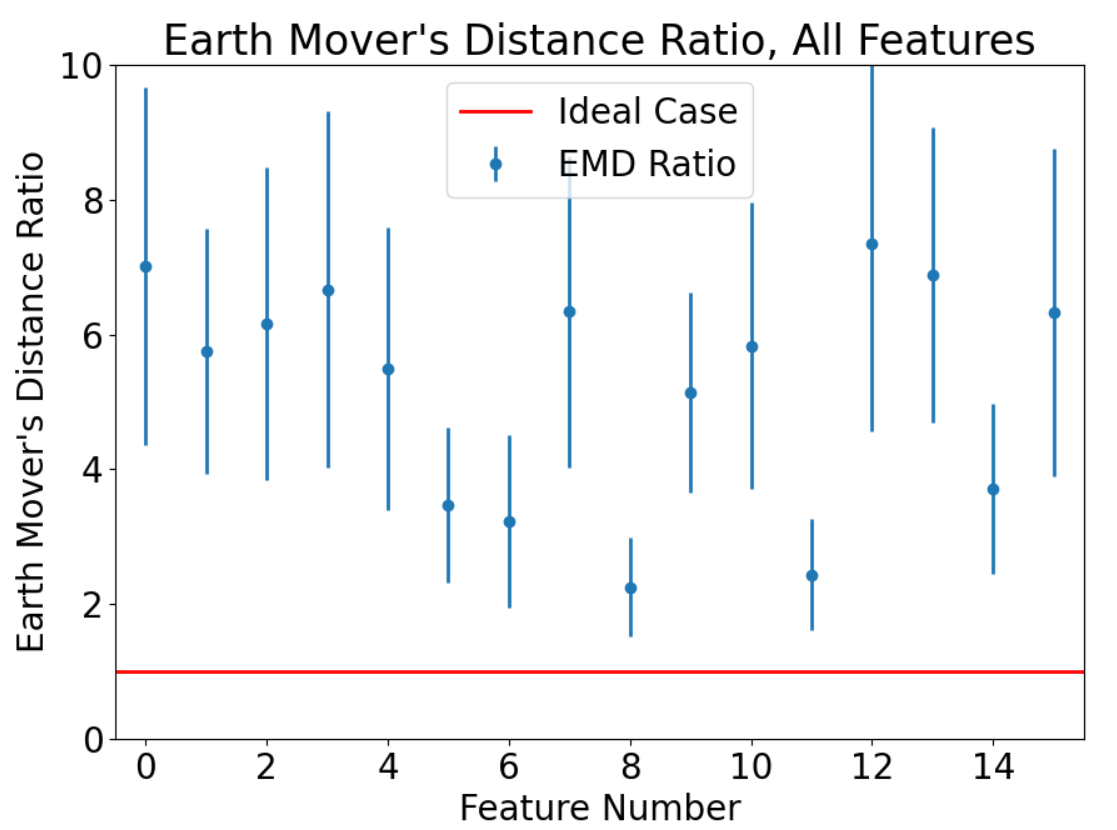
\includegraphics[scale=0.3]{FinalPictures/EMD/EmdRatio.png}
            \label{fig:protons}
        \end{figure}
        
        
        \begin{figure}[H]
            \centering
             \begin{minipage}{0.42349\textwidth}
                \centering
                %Photon 2
                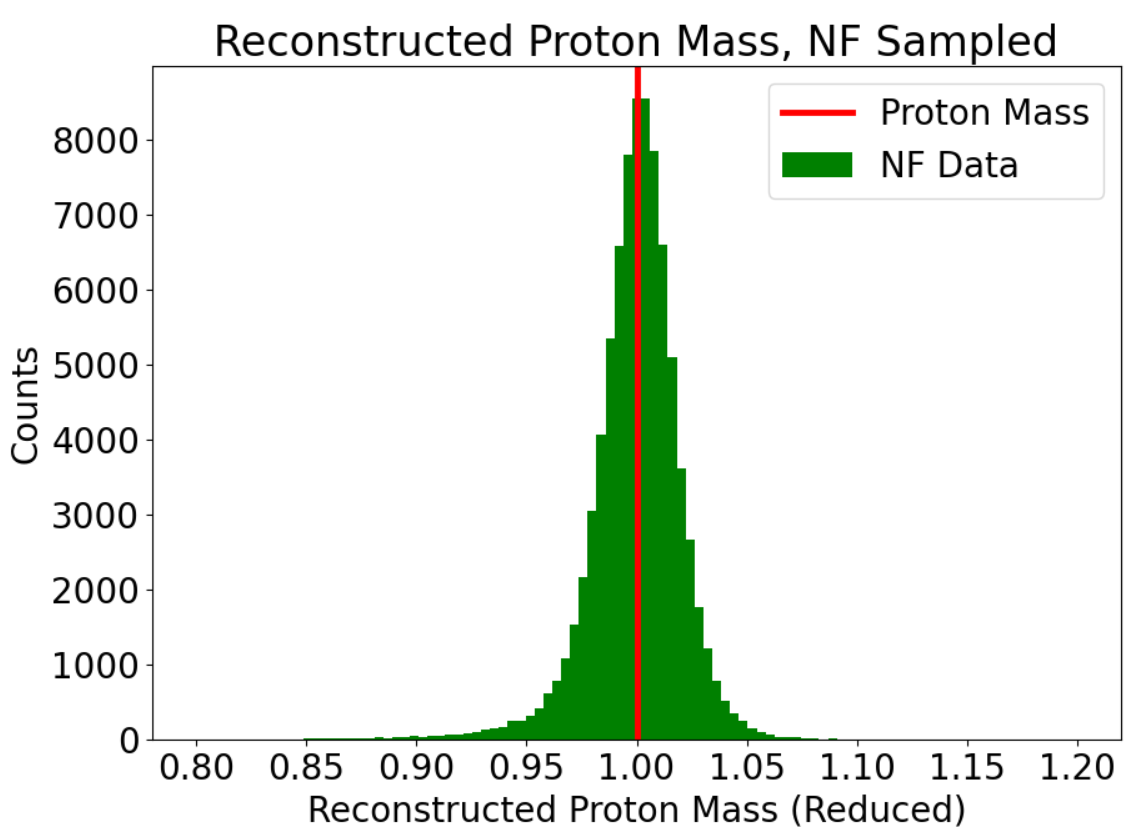
\includegraphics[width=.97\textwidth,trim={ 0 0 0 0},clip]{Chapters/Ch3-Simulations/normalizing_flows/pics/FinalPictures/updated_proton_reduced.png}
        
            \end{minipage}
            \begin{minipage}{0.421245\textwidth}
                \centering
                %Photon 2
                
                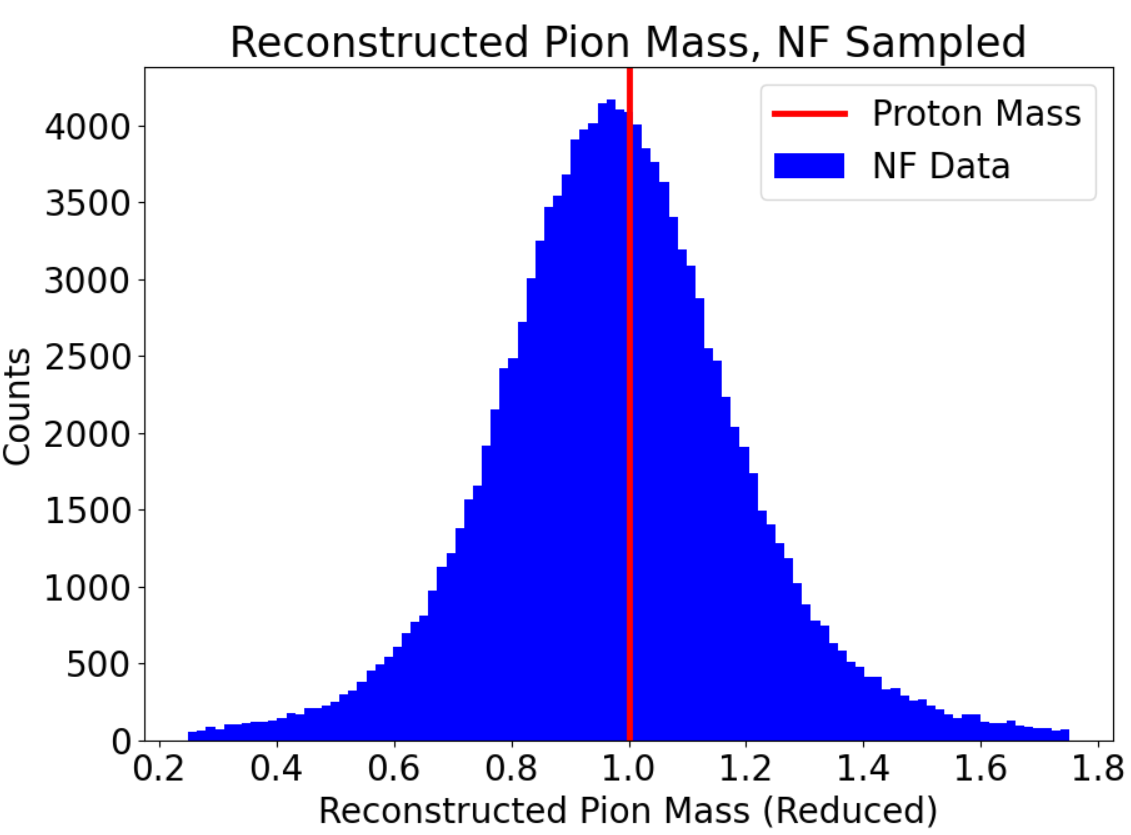
\includegraphics[width=.97\textwidth,trim={ 0 0 0 0},clip]{Chapters/Ch3-Simulations/normalizing_flows/pics/FinalPictures/updated_pion_reduced.png}
            \end{minipage}
                \caption[Generated Proton and Pion Mass Distributions]{The distributions of calculated proton mass (left) and pion mass (right) from the 16-Feature trained NF model.  The accepted (true) particle masses are indicated by the red vertical lines, at 0.938 GeV and 0.135 GeV, respectively.
                The peaks from the model are about 1 MeV, or about 0.5\%, shifted away from these true values; while this is small, it is currently unclear what is causing this shift.}
            \label{fig:protonspions}
        \end{figure}
        

        Finally, investigations were also made into the viability of training 4-feature models rather than the full 16-feature distribution. The 4-feature models were expected to perform better on generating single-particle features than the 16-feature model, but worse when generated data from separate 4-feature models (each corresponding to an individual particle) were combined as the models would lack inter-particle information. Instead, \figref{fig:combined_pion_comparison} (a) shows that the photon-photon invariant mass spectrum for two 4-feature models each trained on a respective photon dataset does a better job of approximating the traditional simulated distribution than the full 16-feature mode. 
        
        \begin{figure}[H]
            \centering
            \subfloat[]{
            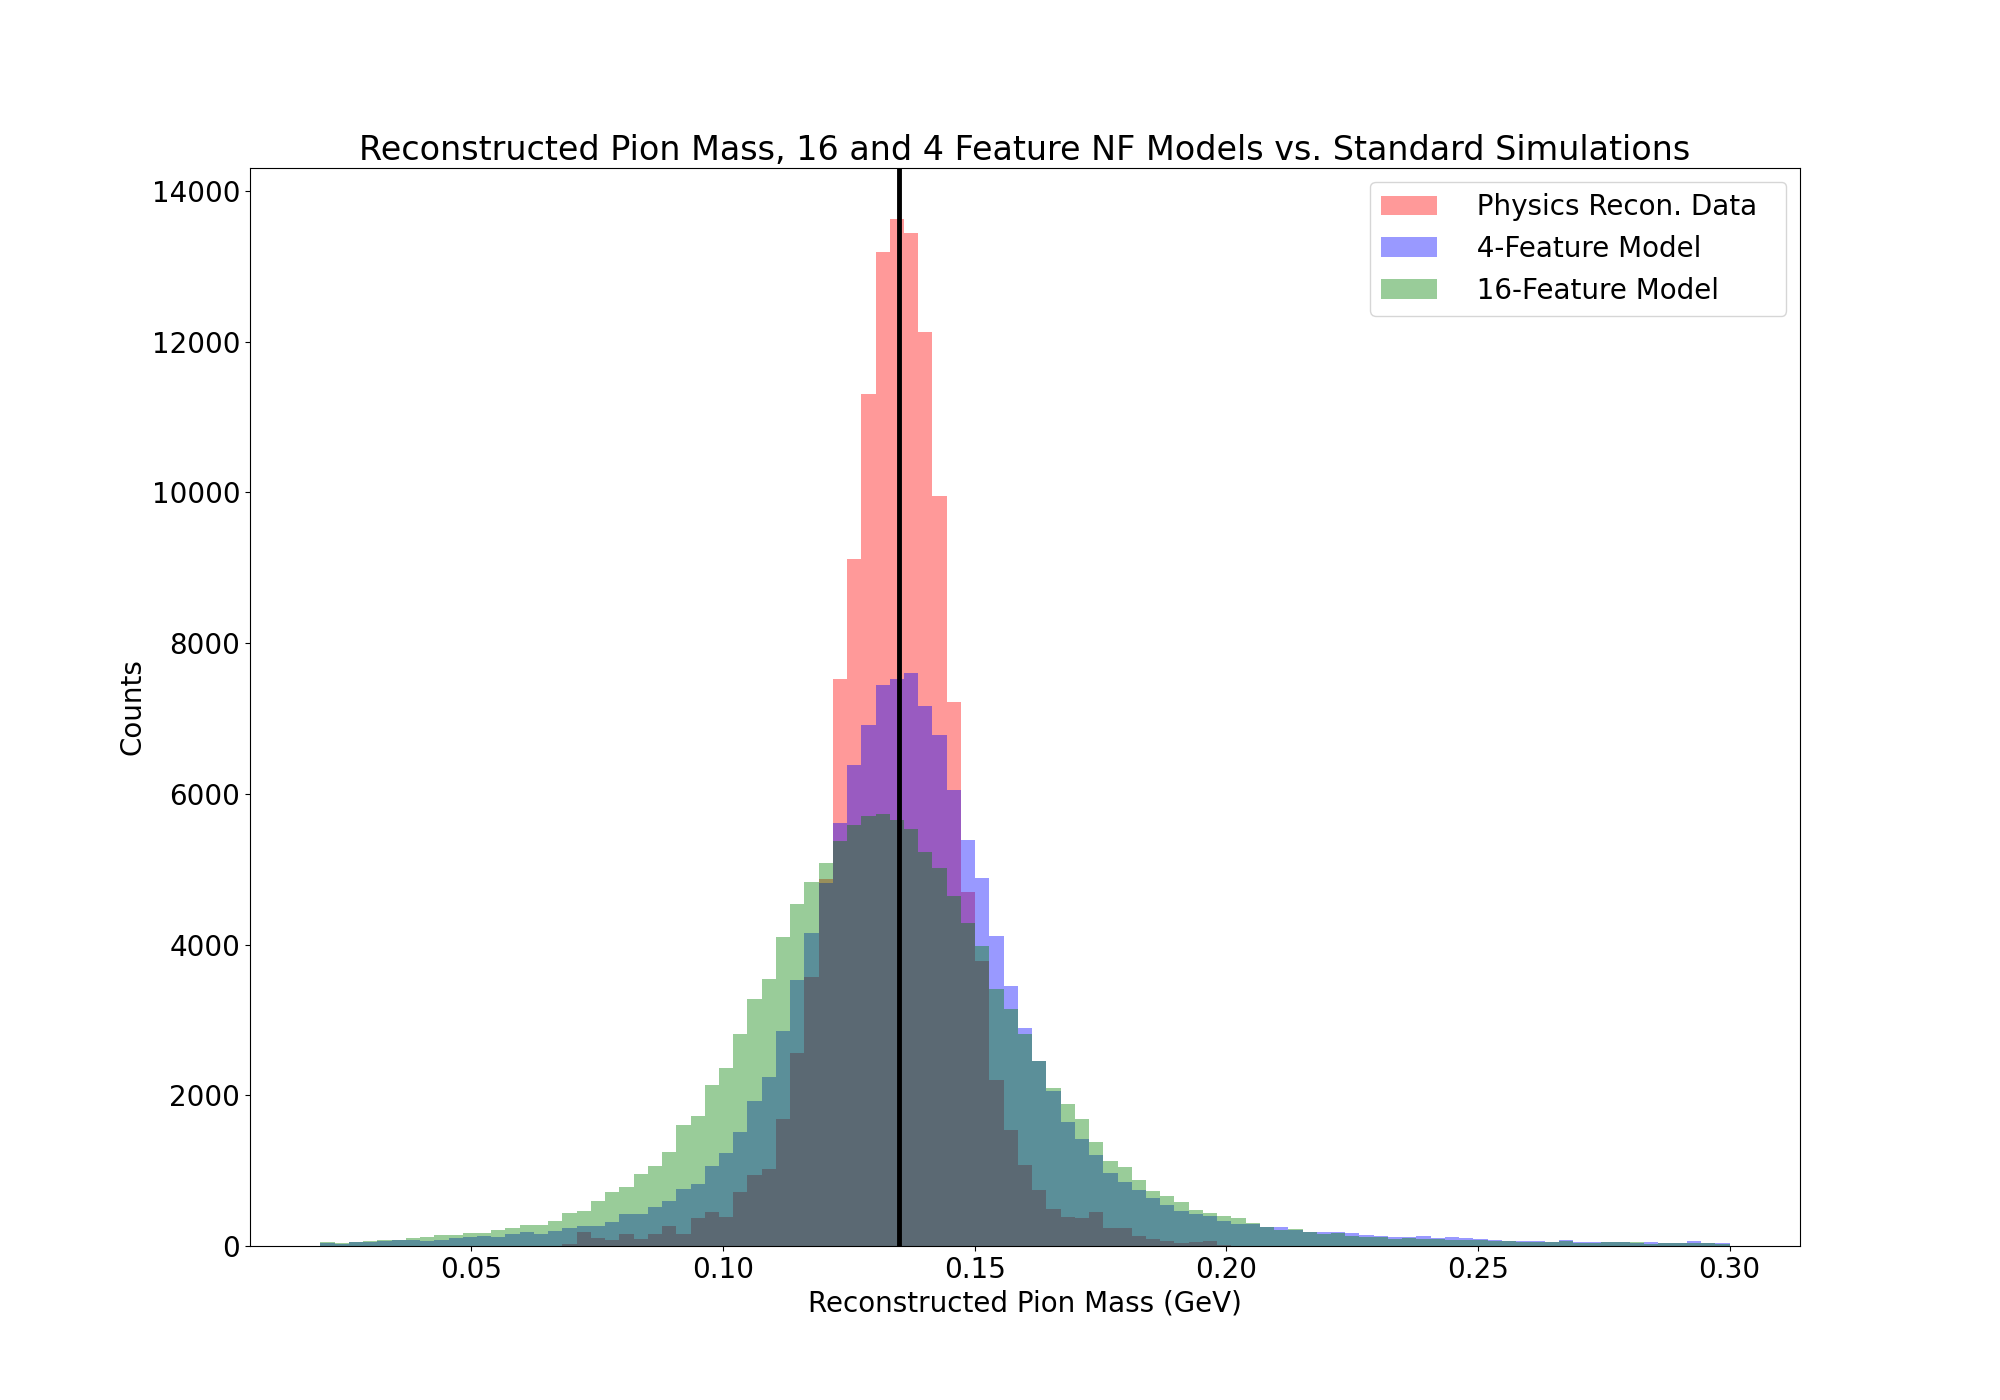
\includegraphics[width = 0.5\textwidth]{Chapters/Ch3-Simulations/normalizing_flows/pics/MeetingFigures/Bobby/Reconstructed_Pion_Mass,_16_and_4_Feature_NF_Models_vs_Standard_Simulations.png}
            \label{fig: jul8_pion_comparison5}
            }
            \hfill
            \subfloat[]{
            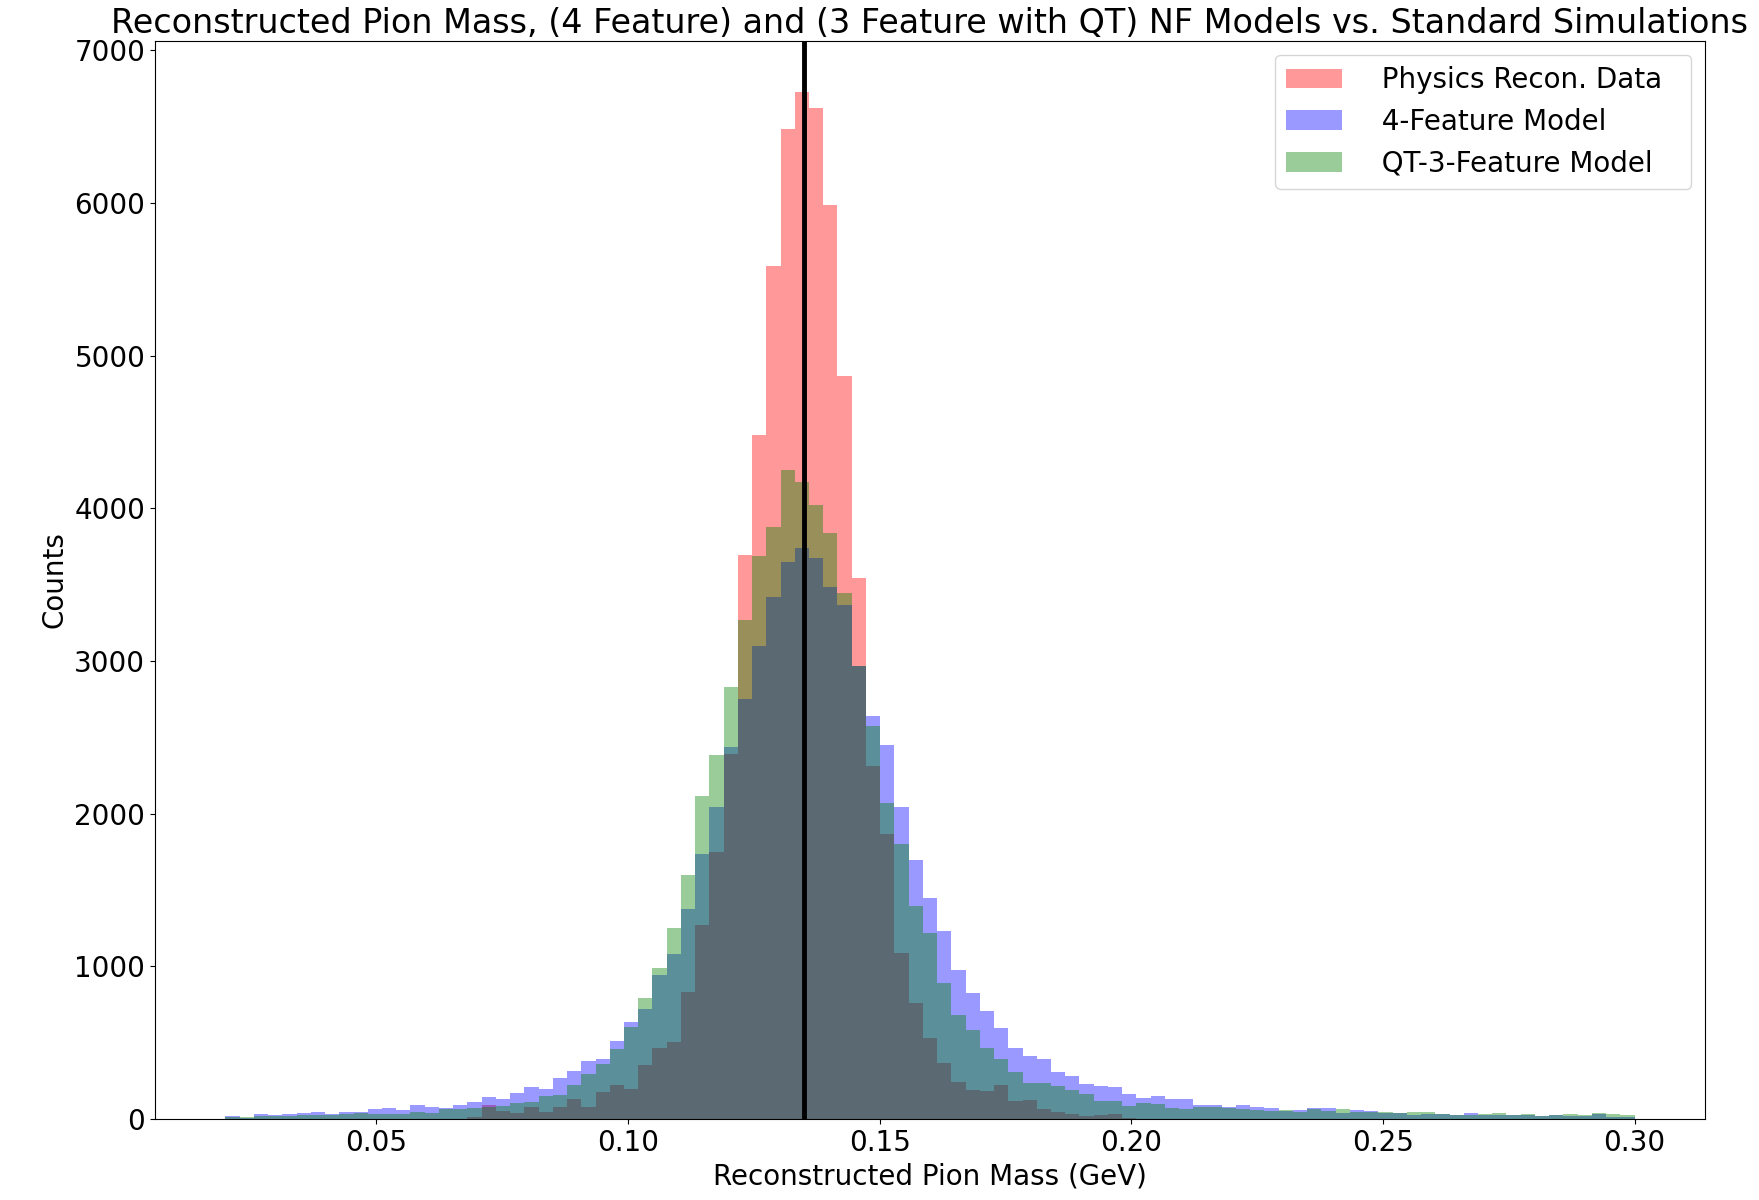
\includegraphics[width = 0.45\textwidth]{Chapters/Ch3-Simulations/normalizing_flows/pics/MeetingFigures/Bobby/qt-3-4.png}
            \label{fig: jul8_pion_comparison}
            }
            \caption[Reconstructed Pion Mass Distributions]{Comparison of reconstructed pion mass with different training models and preprocessing methods. The left panel shows the approximation of the standard reconstruction pion mass peak using a 4 feature model and a 16 feature model, where the 4 feature model shows a better fit. The right panel demonstrates a slight improvement in the reproduction of the GEANT4 simulated pion peak when preprocessing the feature set with a quantile transformer before training the normalizing flow.}
            \label{fig:combined_pion_comparison}
        \end{figure}



\subsection{Summary and Applications}

 Overall, we are able to use a UMNN-MAF architecture to attain reasonable physics distributions far faster than just using traditional physics simulations, with reasonably high fidelity. Unfortunately, there is not a known way to generalize to cases where generated particles are not detected and reconstructed, so it is not immediately useful as a bootstrap on acceptance correction terms. Moreover, statistical uncertainty will not be improved on at an individual level beyond that of the model training, but empirical evidence \parencite{Radhakrishnan2020OverparameterizedMemory} suggests this modeling allows for better interpolation than what would be traditionally expected. 
 
 As the model is trained to understand the transform between the generated and final reconstructed distributions at the particle level, we suspect these techniques ultimately have utility and this effort is ongoing in the CLAS collaboration, but for cross section analysis presented in the rest of this work, we do not utilize data generated by the normalizing flow model.  
 




 \iffalse
Inverse problems

Mike is technically correct that you can't improve the formal statistical uncertainty by training a generic generative model.  But empirically, there is evidence that specific generative models are much better at interpolating than you might have otherwise thought, such that the effective statistical power is higher for the generative output than the original training data  The reason for this improvement isn't fully understand, though.
 
 At this stage, it is not clear if the 10x speedup afforded by the 16-feature NF model is sufficiently large to justify a decrease in fine-detail resolution. Work is ongoing as to if the model resolution can be improved by including conservation laws as part of training, or if the model can be optimized to generate samples faster. 
        
        On the other hand, the 4-feature model has both higher resolution, and is able to produce samples 1,000 times faster than traditional methods, and so could be very useful immediately to physics research efforts. However, as it is only 4-features, it can only represent one particle, not an entire physics process, but this is still relevant to the study of background processes and noise events in physics experiments, and we are investigating applying this to current CLAS12 research.
        
        The ability of the 16-Feature model to produce realistic protons and pions demonstrates viability for using this method in real physics analysis, but we show there are fine details that the model cannot learn without additional constraints. Work is ongoing to incorporate the physical experimental layout and physics conservation laws into the flow training, which we expect will resolve these discrepancies in fine-detail reproduction, and will lead to a more accurate reproduction of the traditional simulation results, at a far faster speed. 

    The conditional normalizing flow takes the base distribution $Y$ and the context $Z$ to learn $X$. How do training and sampling work? 


So this implies that the conditional NF works really well in terms of reproducing collective behavior, but not in the event by event basis that is required for this study. Actually, there is no feature that is directly related to the signs of $x-b$.
    
    
    
    inverse is an ongoing study
    
    We demonstrate a proof of principle for using a normalizing flow to learn a physics process's probability distribution in order to decrease physics simulation computing time and requirements. In this work, we used traditional physics simulations to generate a dataset $\mathbf{x}$ of 5 million data points with each data point having 16 or 4 features.  We take as input a constant 16D or 4D normal distribution $p(\mathbf{z})$, and examine whether the flow model can learn the transformation to $p(\mathbf{x})$ using a random subset of $\mathbf{x}$ for training. We observed a reasonable agreement between the results of the flow-based modeling and traditional physics methods while achieving a computational speedup factor of 10 to 1,000, but the flow is currently unable to reproduce some fine-detailed structures of the physics process.
    
    
    \parencite{Radhakrishnan2020OverparameterizedMemory}

    We show that we can quickly apply realsitc transforms from truth datasets into realistic ones, but exact applicaitons aren't obvious. This remains an ongoing effort, but for the cross section analysis presented in the rest of this work do not utilize data generated by the normalizing flow model. 


    The problem here is that if you use 1M protons to learn a generative model (flow, GAN, etc), then you generate another 19M protons — your statistical error should be roughly the same as you had in the 1M proton sample. You don’t gain information from the generative model — unless there is some additional info that you’re inputing into the model.

    Then, instead of generating particles from scratch for every process studied at LHCb — which is what we do now, i.e. for each analysis people generate MC for that process — for other processes we can use the flow to generate the high-level per-particle features, since the ECAL info for an electron produced in one process is the same as another, provided the flow considers event occupancy and we exclude cases where other particles from the signal process hit the ECAL at the same spot as this electron.

    So, in your case, if somebody has already generated 20M CLAS12 events with your particles, you could learn a flow there, then apply that flow to your reaction in some way. It depends on what specifically you want to simulate or not simulate. In the LHCb case, we were still doing the tracking in the full MC, only adding the ECAL, RICH, and MUON info using the flow. 


    Mike is technically correct that you can't improve the formal statistical uncertainty by training a generic generative model.  But empirically, there is evidence that specific generative models are much better at interpolating than you might have otherwise thought, such that the effective statistical power is higher for the generative output than the original training data  The reason for this improvement isn't fully understand, though.


    In any case, I think this can still be useful if I shift the goal a bit in light of what you said above. In particular, I think the use case would be similar to Constatin's - what I'm simulating is a background process that many collaborators are interested in,  so rather than 50 collaborators simulating 20M events each, it sounds like it could be useful to simulate 20M of these specific events once, train a generative model with it, and then let everyone else generate their sample data from it. (provided the model can work well enough)
    
    Yeah, you just need to make sure that what you’re generating factorizes such that what you learn in one sample can be transferred to another. The easiest way to do this is to not try and learn the kinematical distributions, since they depend on the process — just learn that given a particle of a given type with a given kinematics how to generate all high-level features that your full MC gives you


    \fi
    

    \iffalse
    \begin{figure}[H]
        \centering
        \begin{minipage}{.5\textwidth}
        
            \centering
           % Electron
            
            %\caption[Placeholder Short text]{(a)}
            \includegraphics[width=.99\textwidth,trim={0 0 0 0},clip]{Chapters/Ch3-Simulations/normalizing_flows/pics/MeetingFigures/Bobby/inverse/gen_Px_1_vs_gen_-_recon_Px_1.png}
            \includegraphics[width=.99\textwidth,trim={0 0 0 0},clip]{Chapters/Ch3-Simulations/normalizing_flows/pics/MeetingFigures/Bobby/inverse/gen_Px_1_vs_gen_-_nf_Px_1.png}
    
            %\caption[Placeholder Short text]{(c)}
        \end{minipage}%
        \begin{minipage}{.5\textwidth}
        
            \centering
           % Electron
            
            %\caption[Placeholder Short text]{(a)}
            \includegraphics[width=.99\textwidth,trim={0 0 0 0},clip]{Chapters/Ch3-Simulations/normalizing_flows/pics/MeetingFigures/Bobby/inverse/gen_Py_1_vs_gen_-_recon_Py_1.png}
            \includegraphics[width=.99\textwidth,trim={0 0 0 0},clip]{Chapters/Ch3-Simulations/normalizing_flows/pics/MeetingFigures/Bobby/inverse/gen_Py_1_vs_gen_-_nf_Py_1.png}
    
            %\caption[Placeholder Short text]{(c)}
        \end{minipage}%
        \caption[Placeholder Short text]{\textbf{TOP:} Truth Event - Reconstructed Event. If standard physics reconstruction algorithms were perfect, we would have a horizontal line at 0 across the distribution (no difference between the reconstructed feature value, and the true feature value, for any event in the data set). \textbf{BOTTOM:} Truth Event - NF estimate of truth event conditional on Reconstructed event values. For the NF to be useful, we would need the difference between the truth event values and the NF estimates to be closer to zero than the differences between just the truth and reconstructed values. However, instead we observe that the spread is about a factor of 2 \textbf{worse} using the NF than not using it at all. }
        \label{fig:16features6}
    \end{figure}
    \fi
    
    
    
    
    
    \iffalse
    From Mike Williams


    You could instead enforce the conservation law in the normalizing flow, which is what I would do if I wanted to use something like this — but perhaps not do if you’re simply trying to show that you can approximately learn the conservation law. So, depends on the goal. 

    Ultimately, since we know how to quickly simulate kinematics, I think what Constantin did with learning to simulate detector features is the most useful thing for a real-world application, but again depends on what your goals are.




    \fi